\documentclass[oneside]{book}

\usepackage{ifthen}
\newboolean{draft}
\setboolean{draft}{false}
\newcommand{\IfDraft}[1]{\ifthenelse{\boolean{draft}}{#1}{}}
\newcommand{\IfNotDraft}[1]{\ifthenelse{\boolean{draft}}{}{#1}}

\usepackage[utf8]{inputenc}
\usepackage[T1]{fontenc}
\usepackage[russian]{babel}
\usepackage[a4paper]{geometry}
\usepackage[usenames,dvipsnames]{color}
\usepackage[svgnames,dvipsnames]{xcolor}

\usepackage{tikz}
\usetikzlibrary{arrows,backgrounds,calc,positioning,trees}
\usepackage{pgfplots}

\usepackage{graphicx}

\usepackage{indentfirst}
\usepackage{booktabs}
\usepackage{amsmath}
\usepackage{amsfonts}
\usepackage{caption}
\usepackage{listings}
\usepackage{hyperref}
\usepackage{varioref}
\usepackage{enumerate}
\usepackage{epigraph}

\hypersetup{
  colorlinks,
  citecolor=black,
  filecolor=black,
  linkcolor=black,
  urlcolor=black
}

\newenvironment{epistyle}{\setlength{\parindent}{1em}}{}
\renewcommand{\textflush}{epistyle}

\DeclareCaptionFont{white}{\color{white}}
\DeclareCaptionFormat{listing}{\colorbox{Gray}{\parbox{\textwidth}{\hspace{15pt}#1#2#3}}}

\captionsetup[lstlisting]{
  format=listing,
  labelfont=white,
  textfont=white,
  singlelinecheck=false,
  margin=0pt,
  font={bf,footnotesize}}

\lstset{
  basicstyle=\footnotesize\ttfamily,
  numbers=left,
  numberstyle=\tiny,
  stepnumber=5,
  numbersep=5pt,
  tabsize=2,
  extendedchars=true,
  keywordstyle=\color{PineGreen},
  commentstyle=\color{NavyBlue},
  stringstyle=\color{Orange},
  xleftmargin=25pt,
  breaklines=true,
  breakatwhitespace=false,
  showspaces=false,
  showtabs=false,
  captionpos=t,
}

\lstdefinestyle{plainstyle}{language=}
\lstnewenvironment{plainlst}[2]
  {\lstset{style=plainstyle,caption=#1,label=#2}}
  {}

\lstdefinestyle{cstyle}{language=C}
\lstnewenvironment{clst}[2]
  {\lstset{style=cstyle,caption=#1,label=#2}}
  {}

\lstdefinestyle{pystyle}{language=Python,mathescape}
\lstnewenvironment{pylst}[2]
  {\lstset{style=pystyle,caption=#1,label=#2}}
  {}

\lstdefinestyle{ocamlstyle}{language=[Objective]Caml,mathescape}
\lstnewenvironment{ocamllst}[2]
  {\lstset{style=ocamlstyle,caption=#1,label=#2}}
  {}

\lstdefinestyle{hsstyle}{language=Haskell}
\lstnewenvironment{hslst}[2]
  {\lstset{style=hsstyle,caption=#1,label=#2}}
  {}

\lstdefinestyle{clstyle}{language=Lisp}
\lstnewenvironment{cllst}[2]
  {\lstset{style=clstyle,caption=#1,label=#2}}
  {}

\title{Informatics Rescue}
\author{Вадим Шендер, Иван Чернецкий}

\begin{document}
\maketitle{}

\tableofcontents{}

\chapter{Базовые структуры данных и алгоритмы}
\label{ch:basic-ds}

\section{О-нотация}
\section{Двоичный поиск}
\section{Сортировка}
\section{Расширяемые массивы}
\section{Списки}
\section{Деревья}
\section{Хэш-таблицы}
\section{Динамическое программирование}
\section{Некоторые заметки о языке C}

\chapter{Язык программирования Python}
\label{ch:python}

\section{Типы и структуры данных и операции над ними}
\label{sec:py-types}
Python --- динамически типизированный язык. Типы принадлежат объектам, не переменным. Переменные лишь связываются с объектами. Python --- строго типизированный язык. Все типы проверяются во время исполнения. Если обнаруживается какое-либо несоответствие типов, то возникает исключение \lstinline{TypeError}.

Все объекты деляется на ссылочные и атомарные. При присваивании атомарных объектов они копируются, в то время как при присваивании ссылочных объекто копируюся только ссылки на них. Ссылочные объекты могут быть изменяемыми или неизменяемыми (mutable и immutable, соответственно).

\subsection{NoneType}
Единственным экземпляром этого типа является \lstinline{None}. Используется для обозначение того факта, что значения нет, например, ``функция ничего не возвращает''. С \lstinline{None} можно использовать операции сравнения и т.п.

\subsection{Булев тип}
\lstinline{False} -- ложное значение булева типа, а \lstinline{True} --- истинное значение.

Любой объект может быть проверен на истинность (как все просто!) для использования в операторах \lstinline{if} и \lstinline{while}. Следующие значения считаются ложными:
\begin{itemize}
  \item \lstinline{None};
  \item \lstinline{False};
  \item нуль любого числового типа;
  \item любая пустая последовательность;
  \item любое пустое отображение (словарь);
  \item экземпляр класса, определенного пользователем, если в классе определены \lstinline{__nonzero__()} или \lstinline{__len()} методы, и они возвращают нуль или \lstinline{False}.
\end{itemize}

Все остальные значения считаются истинными.

\subsubsection{Булевы операции}
\begin{center}
  \begin{tabular}{lp{6cm}}
    \toprule
    Операция & Результат \\
    \midrule
    x or y & Если x истинен, то x, иначе y. \\
    x and y & Если x истинен, то y, иначе x. \\
    not x & Если x истинен, то False, иначе True. \\
    \bottomrule
  \end{tabular}
\end{center}

\subsection{Числовые типы}
Четыре числовых типа: \lstinline{int}, \lstinline{long}, \lstinline{float} и \lstinline{complex}. \lstinline{int} соответсвует \lstinline{long} языка C. Для типа \lstinline{long} языка Python нет ограничений на размер числа. \lstinline{float} языка Python реализован с помощью типа \lstinline{double} языка C. Комплексные числа имеют действительную и мнимую составляющие, каждая из которые представлена \lstinline{double} языка C.

\begin{pylst}{Работа с числовыми типами}{}
>>> x, y = 5, 7
>>> x + y, x / y, y % x
12, 0, 2
>>> x ** y ** 2
17763568394002504646778106689453125L
>>> abs(-x)
5
>>> x, y = 3.5, 23.3
>>> round(x), y / x
4.0, 6.6571428571428575
>>> z = 1.3 + 0.5j
>>> z.imag
0.5
\end{pylst}

Python предоставляет все стандартные побитовые операции над целыми числами: \lstinline{|} (побитовое ИЛИ), \lstinline{^} (побитовое ИСКЛЮЧАЮЩЕЕ ИЛИ), \lstinline{&} (побитовое И), \lstinline{<<} (сдвиг влево), \lstinline{>>} (сдвиг вправо) и \lstinline{~} (побитовое НЕ).

\subsection{Последовательности}
Четыре типа последовательности: \lstinline{string} (строки), \lstinline{unicode} (юникодные строки), \lstinline{list} (списки), \lstinline{tuple} (кортежи).

Все последовательности поддерживают следующие операции:
\begin{center}
  \begin{tabular}{lp{7.5cm}}
    \toprule
    Операция & Результат \\
    \midrule
    \texttt{x in s} & Истина, если какой-либо элемент из \texttt{s} равен \texttt{x} \\
    \texttt{x not in s} & Истина, если ни один элемент из \texttt{s} не равен \texttt{s} \\
    \texttt{s + t} & Сцепка \texttt{s} и \texttt{t} \\
    \texttt{s * n} & Сцепка \texttt{s} с собой \texttt{n} раз \\
    \texttt{s[i]} & Доступ по индексу \texttt{i} \\
    \texttt{s[i:j]} & Срез от \texttt{i} до \texttt{j} \\
    \texttt{s[i:j:k]} & Срез от \texttt{i} до \texttt{j} с шагом \texttt{k} \\
    \texttt{len(s)} & Длина \texttt{s} \\
    \texttt{min(s)} & Минимальный элемент в \texttt{s} \\
    \texttt{max(s)} & Максимальный элемент в \texttt{s} \\
    \bottomrule
  \end{tabular}
\end{center}

\begin{pylst}{Работа с последовательностями}{}
>>> s = 'not so long string '
>>> 'l' in s, 'l' not in s
True, False
>>> s + '...'
'not so long string ...'
>>> s * 2
'not so long string not so long string '
>>> s[10], s[1:6], s[1:9:2]
'g', 'ot so', 'o ol'
>>> len(s)
19
\end{pylst}

\subsubsection{Строки}
Строка в Python --- неизменяемый тип данных. Все операции над последовательностями работают и со строками. Ниже проиллюстрированы часто употребляемые методы:
\begin{pylst}{}{}
>>> s = 'In the very beginning...'
>>> s.count('in')
2
>>> s.startswith('in')
False
>>> ', '.join(['a', 'b', 'c'])
'a, b, c'
>>> s.upper()
'IN THE VERY BEGINNING...'
>>> s.partition(' ')
('In', ' ', 'the very beginning...')
>>> s.split(' ')
['In', 'the', 'very', 'beginning...']
>>> '%s there was actually nothing' % s
'In the very beginning... there was actually nothing'
\end{pylst}

Строковые литералы могут быть трёх видов:
\begin{itemize}
  \item \lstinline{'string'} или \lstinline{"string"}.
  \item \lstinline{'''string'''} или \lstinline{"""string"""}. Может занимать несколько строк.
  \item \lstinline{r'string'} или \lstinline{r"string"}. Специальные символы не надо экранировать.
\end{itemize}

\subsubsection{Списки}
Список в Python --- изменяемая структура данных. Все операции над последовательностями применимы и к спискам. В таблице~\ref{tbl:py-listops} приведены некоторые операции, специфичные для списков.
\begin{table}[h!]
  \begin{center}
    \caption{Дополнительные операции над списками\label{tbl:py-listops}}
    \begin{tabular}{lp{9cm}}
      \toprule
      Операция & Результат \\
      \midrule
      \texttt{s[i] = x} & Замещает элемент на позиции \texttt{i} переменной \texttt{x} \\
      \texttt{s[i:j] = t} & Срез от \texttt{i} до \texttt{j} замещается содержимым итератора \texttt{t} \\
      \texttt{del s[i:j]} & То же, что и \texttt{s[i:j] = []} \\
      \texttt{s[i:j:k] = t} & Элементы \texttt{s[i:j:k]} замещаются содержимым \texttt{t} \\
      \texttt{del s[i:j:k]} & Удаляет элементы \texttt{s[i:j:k]} из списка \\
      \texttt{s.append(x)} & Добавляет элемент в конец списка \\
      \texttt{s.extend(x)} & То же самое, что и \texttt{s[len(s):len(s)] = x} \\
      \texttt{s.insert(i, x)} & То же самое, что и \texttt{s[i:i] = [x]} \\
      \texttt{s.pop([i])} & То же самое, что и \texttt{x = s[i]; del s[i]; return x} \\
      \texttt{s.remove(x)} & То же самое, что и \texttt{del s[s.index(x)]} \\
      \bottomrule
    \end{tabular}
  \end{center}
\end{table}

\subsubsection{Кортежи}
Кортеж --- это неизменяемая последовательность элементов. Нельзя ни удалять элементы из кортежа, ни добавлять, ни изменять. Примеры создания кортежей:
\begin{pylst}{}{}
>>> tuple([1, 2, 3])
(1, 2, 3)
>>> ('a', 'b', 'c')
\end{pylst}

\subsection{Словари}
Словарь --- изменяемая структура данных. Он отображает хешируемые значения на любые объекты.
\begin{pylst}{Примеры создания словаря}{}
dict(one=2, two=3)
dict({'one': 2, 'two': 3})
dict(zip(('one', 'two'), (2, 3)))
dict([['two', 3], ['one', 2]])
\end{pylst}

Некоторые операции над словарём \texttt{d}:
\begin{itemize}
  \item \lstinline{d[key]}. Возвращает объект, ассоциированный с ключом \lstinline{key}. Если такового нет --- \lstinline{KeyError}.
  \item \lstinline{d[key] = value}. Ассоциирует объект \lstinline{value} с ключом \lstinline{key}.
  \item \lstinline{del d[key]}. Удаляет объект, ассоциированный с ключом \lstinline{key}.
  \item \lstinline{key in d}. \lstinline{True}, если \lstinline{d} имеет ключ \lstinline{key}.
  \item \lstinline{key not in d}. Обратно.
  \item \lstinline{iter(d)}. Возвращает итератор по ключам словаря.
  \item \lstinline{clear()}. Удаляет все элементы из словаря.
  \item \lstinline{items()}. Возвращает список пар вида \lstinline{(key, value)}.
  \item \lstinline{iteritems()}. Возвращает итератор по \lstinline{items()}.
  \item \lstinline{iterkeys()}. Возвращает итератор по ключам.
  \item \lstinline{itervalues()}. Возвращает итератор по ассоциированным объектам.
  \item \lstinline{keys()}. Список всех ключей.
  \item \lstinline{values()}. Список ассоциированных объектов.
  \item \lstinline{update([other])}. Обновляет словарь элементами словаря \lstinline{other}.
\end{itemize}

\subsection{Множества}
Очень похожи на математические множества. Поддерживает операции объединения, пересечения, вычитания и различные проверки. Некоторые операции:
\begin{itemize}
  \item \lstinline{isdisjoint(other)}. Возвращает \lstinline{True}, если множества не имею одинаковых элементов.
  \item \lstinline{issubset(other)} или \lstinline{set <= other}. Проверяет, все ли элементы первого множества присутствуют во втором.
  \item \lstinline{issuperset(other)} или \lstinline{set >= other}. По аналогии.
\end{itemize}

\section{Операторы}
\label{sec:py-statements}

\subsubsection{Оператор if}
Общая форма оператора \lstinline{if} выглядит следующим образом:
\begin{pylst}{}{}
if $expression$: $suite$
( elif $expression$: $suite$)*
[ else: $suite$ ]
\end{pylst}

Этот оператор вычисляет последовательно выражения $expression$ до тех пор, пока не будет найдено равное \lstinline{true}. После чего выполняется соответсвующее $suite$. Если все выражения оказались равными \lstinline{false}, то выполняются операторы и выражения из \lstinline{else} ветки. Выполняется не больше одного набора операторов и выражений ($suite$).

\subsubsection{Оператор while}
Общая форма оператора \lstinline{while} выглядит следующим образом:
\begin{pylst}{}{}
while $expression$: $suite_1$
[ else: $suite_2$ ]
\end{pylst}

Выполняет $suite_1$ пока $expression$ истинно. Если в первый раз $expression$ оказалось ложно, выполняется ветка \lstinline{else}, после чего цикл завершается. Оператор \lstinline{break} завершает цикл без выполнения ветки \lstinline{else}. Оператор \lstinline{continue} передает управление на начало цикла.

\subsubsection{Оператор for}
Общая форма оператора \lstinline{for} выглядит следующим образом:
\begin{pylst}{}{}
for $variable$ in $expression$: $suite_1$
[ else: $suite_2$ ]
\end{pylst}

$expression$ вычисляется единожды. Оно должно вычислятся в итерируемый объект. Затем $suite_1$ вычисляется столько раз, сколько объектов в итерируемом объекте, при этом переменной $variable$ присваивается очередной объект. По завершении вычисляется ветка \lstinline{else}.

Оператор \lstinline{break} завершает цикл без выполнения ветки \lstinline{else}. Оператор \lstinline{continue} передает управление на начало цикла или, если больше нет очередного объекта, на ветку \lstinline{else}.

\subsubsection{Оператор try}
Общая форма оператора \lstinline{try} выглядит следующим образом:
\begin{pylst}{}{}
try: suite
( except [expression [ ( as | "," ) target ] ]: suite )+
[ else: suite ]
[ finally: suite ]
\end{pylst}
или
\begin{pylst}{}{}
try: suite
finally: suite
\end{pylst}

Блоки \lstinline{except} определяют обработчики исключительных ситуаций. Если в блоке \lstinline{try} не возникло исключительной ситуации, то ни один из обработчиков не выполняется. В ином случае происходит поиск подходящего обработчика последовательно по блокам \lstinline{except}. Блок \lstinline{except} без выражений $expression$, если таковой присутствует, должен быть последним. При поиске выражения $expression$ вычисляются, и блок выбирается для выполнения, если объект-результат подходит к возникшему исключению, т.е. если объект является классом, который присутствует в списке наследования объекта исключения, или же кортежем, в котором хотя бы один элемент является совместимым с исключением.

Если обработчик не найден, поиск происходит в обрамляющем коде и вверх дальше по стеку, если блок \lstinline{finally} не присутсвует.

Если при выполнении выражений $expression$ возникло исключение, то изначальное исключение отбрасывается, и начинается новый поиск для нового исключения в обрамляющем коде и вверх по стеку.

Если же подходящий блок \lstinline{except} найден, то $target$, если присутствует, присваивается результат вычисления $expression$, и блок исполняется. После чего управление передается, как правило, за пределы оператора \lstinline{try}.

В блоке обработчика можно вызвать \lstinline{sys.exc_info}, которая возвращает кортеж \lstinline{(exc_type, exc_value, exc_traceback)}, где \lstinline{exc_type} --- объект исключения, \lstinline{exc_value} --- параметры, переданные исключению, \lstinline{exc_traceback} --- traceback объект.

Блок \lstinline{else} выполняется в том случае, если управление достигло конца блока \lstinline{try}. Исключения, возникшие в блоке \lstinline{else} не обрабатываются предыдущими ему обработчиками.

Блок \lstinline{finally} выполняется всегда, где бы исключительная ситуация не возникла: внутри блок \lstinline{try}, \lstinline{except} или же \lstinline{else}.

\section{Функции}
Ниже приведено тривиальное определение функции:
\begin{pylst}{}{}
def add(a, b):
    return a + b
\end{pylst}

Как видно из примера, определение функции начинается с оператора \lstinline{def}, за которым идет имя функции, а следом --- аргументы, заключенные в круглые скобки. Возврат значения происходит посредством оператора \lstinline{return}. Если возврат из функции происходит из-за того, что управление достигло конца функции, то возвращаемое значение равно \lstinline{None}. Определение функции связывает её имя с объектом функции (обёрткой над действительно исполняемым кодом) в текущем пространсве имён. Объект функции содержит ссылку на текущее глобальное пространство имён, которое будет использоваться при вызове функции.

Определение функции может быть обёрнуто декораторами. Декораторы вычисляются во время определения функции в том же самом контексте, где находится определение функции.

Функция может иметь именованные аргументы, которые имеют значение по умолчанию. При вызове функции не обязательно передавать именованные аргументы, если устраивает значение по умолчанию. В определении функции после именованного аргумента могут идти только именованные аргументы.

Значения по умолчанию для именованных аргументов вычисляются один раз при выполнении определения функции. После чего при любом вызове используется один и тот же объект. Если значение по умолчанию --- изменяемый (mutable) объект, то можно наткнуться на неприятности, что и проиллюстрировано ниже:
\begin{pylst}{}{}
def append(list=[]):
    list.append('a')
    return list

>>> append()
['a']
>>> append()
['a', 'a']
>>> append()
['a', 'a', 'a']
\end{pylst}

Ниже представлена версия, лишенная приведенного недостатка:
\begin{pylst}{}{}
def append(list=None):
    if list is None:
        list = []
    list.append('a')
    return list

>>> append()
['a']
>>> append()
['a']
\end{pylst}

Если в определении функции присутствует форма \lstinline{*identifier}, то \lstinline{identifier} будет равен кортежу, который содержит все аргументы, которые не были явно проименованы. Если же присутствует форма \lstinline{**identifier}, то \lstinline{identifier} будет словарём, который отображет имена аргументов на их значения.

При вызове если происходит ошибка разбора аргументов, их нехватка или избыток и так далее, то порождается исключение \lstinline{TypeError}. Если при вызове присутствует форма \lstinline{*identifier}, то \lstinline{identifier} должен вычисляться в последовательность, элементы которой будут считаться дополнительными позиционными аргументами. Если же при вызове присутсвует форма \lstinline{**identifier}, то \lstinline{identifier} должен вычисляться в словарь, ключи которого будут использоваться в качестве именованных аргументов, а значения --- в качестве значений этих аргументов.

Обе формы могут присутствовать одновременно как при определении функции, так и при вызове.

\subsubsection{Анонимные функции}
\emph{Анонимные (безымянные) функции} в Python --- объекты функций, которые не имеют имени ни в каком пространстве имён после \emph{непосредственного} определения. Они определяются с помощью лямбда-выражений:
\begin{pylst}{}{}
lambda [ $parameters$ ]: $expression$
\end{pylst}

В отличии от обычного определения функции лямбда-выражение не может содержать операторов (statements).
\begin{pylst}{}{}
>>> map(lambda i: i + 1, [1, 2, 3])
[2, 3, 4]
\end{pylst}

\section{Функциональное программирование}
В Python возможно использовать некоторые идеи и концепции функционального программирования.

\subsection{Функции высшего порядка}
Функция высшего порядка --- функция, принимающая в качестве аргументов другие функции или возвращающая другую функцию в качестве результата.
\begin{pylst}{}{}
def f(x):
    return x + 3
 
def g(function, x):
    return function(x) * function(x)
 
>>> g(f, 7)
100
\end{pylst}

Ниже представлены наиболее общеупотребимые функции высшего порядка, определенные в Python.

\subsubsection{Функция map}
\lstinline{map} --- функция высшего порядка, которая применяет переданную функция к элементам одной или нескольких последовательностей. Количество аргументов переданной функции должно быть равно количеству переданных последовательностей. Если последовательности не одинаковой длины, то вместо недостающих элементов используется \lstinline{None}. Длина результирующего списка равна длине наибольшего списка. Если вместо функции передается \lstinline{None}, тогда элементы последовательностей никак не преобразуются, а используются как есть. Если последовательностей --- несколько, то результатом будет список кортежей.
\begin{pylst}{}{}
map(function, sequence[, sequence, ...]) -> list

>>> map(lambda x, y: x + y, [1, 2, 3], [2, 3, 4])
[3, 5, 7]
>>> map(None, [1, 2], [3])
[(1, 3), (2, None)]
\end{pylst}

\subsubsection{Функция filter}
\lstinline{filter} --- функция высшего порядка, которая конструирует итоговый список из элементов переданной последовательности, если конкретный элемент удовлетворяет функции-предикату. Если в качестве последовательности передается строка или кортеж, то и тип результата будет строка или кортеж, соответственно. Если функция равна \lstinline{None}, то возвращаются элементы, которые истинны.
\begin{pylst}{}{}
filter(function or None, sequence) -> list, tuple, or string

>>> filter(lambda x: x % 2, [1, 2, 3, 4, 5])
[1, 3, 5]
\end{pylst}

\subsubsection{Функция reduce}
\lstinline{reduce} --- функция высшего порядка, которая делает свёртку последовательности, в результате чего получается, как правило, значение типа элемента последовательности. Функция свёртки обычно принимает три аргумента: комбинирующую функцию \lstinline{function}, начальное значение \lstinline{initial} и последовательность \lstinline{sequence}.
\begin{pylst}{}{}
reduce(function, sequence[, initial]) -> value
\end{pylst}

$4!$ можно вычислить следующим образом, используя функцию \lstinline{reduce}:
\begin{pylst}{}{}
>>> reduce(lambda res, x: res * x, range(2, 4 + 1), 1)
24
\end{pylst}

Вычисление происходит следующим образом:
\begin{center}
  \begin{tikzpicture}[level/.style={sibling distance=50mm/#1}]
    \node [circle, draw] {$*$}
      child { node [circle, draw] {$*$}
        child { node [circle, draw] {$*$} 
          child { node [circle, draw] {$1$} }
          child { node [circle, draw] {$2$} } }
        child { node [circle, draw] {$3$} } }
      child { node [circle, draw] {$4$} };
  \end{tikzpicture}
\end{center}

Другая иллюстрация:
\begin{pylst}{}{}
(((1 * 2) * 3) * 4)
\end{pylst}

\subsection{Рекурсия}
Хоть в Python и существует рекурсия, но в наиболее популярной реализации этого языка --- CPython --- она не православна, так как там нет оптимизации хвостовых вызовов (tail call optimization, TCO).

Хвостовая рекурсия --- специальный случай рекурсии, при котором последней операцией, выполняемой рекурсивной функцией, является вызов самой себя. Подобный вид рекурсии примечателен тем, что может быть легко и автоматически заменён на итерацию, что и делают многие оптимизирующие компиляторы. Подобные рассуждения справедливы и для взаимно рекурсивных функций, хоть TCO для них в компиляторах встречается еще реже.

\begin{pylst}{}{}
def infinite():
    infinite()

# shortly somewhere in a far far away galaxy
>>> infinite()
Traceback (most recent call last):
  File "<stdin>", line 1, in <module>
...
RuntimeError: maximum recursion depth exceeded
\end{pylst}

Получить и установить максимальное возможное количество рекурсивные вызовов можно с помощью функцией \lstinline{sys.getrecursionlimit} и \lstinline{sys.setrecursionlimit(limit)}.

\subsection{Замыкания}
Замыкание --- первоклассная функция со свободными переменными, которые связаны с определенными значениями в своем лексическом окружении. Свободная переменная --- переменная, которая встречается в теле функции, но которая не является параметром этой функции или локальной переменной.
\begin{pylst}{}{}
def make_adder(y):
    def add(x):
        return x + y
    return add

>>> add5 = make_adder(5)
>>> add5(5)
10
>>> add5(7)
12
\end{pylst}

Замыкание \lstinline{add} создается при каждом вызове функции \lstinline{make_adder}. Замыкании \lstinline{add} переменная \lstinline{y} является свободной переменной.

Замыкания в Python также не доведены до логического конца, хоть в версиях $>=3.0$ уже такая претензия есть. В версии 3.0 введен оператор \lstinline{nonlocal}, суть которого видна из следующего примера:
\begin{pylst}{}{}
def make_counter():
    count = 0
    def get():
        return count
    def inc():
        count += 1

    return get, inc

>>> get, inc = make_counter()
>>> get()
>>> 0
>>> inc()
Traceback (most recent call last):
  File "<stdin>", line 1, in <module>
  File "/tmp/py9637pml", line 11, in inc
UnboundLocalError: local variable 'count' referenced before assignment

def make_counter():
    count = 0
    def get():
        nonlocal count
        return count
    def inc():
        count += 1

    return get, inc

>>> get, inc = make_counter()
>>> get()
>>> 0
>>> inc()
>>> get()
1
\end{pylst}

\subsection{Частичное применение функции}
Частичное применение функции --- это преобразование функции от $n$ аргументов к функции от $n - m$ аргументов ($m < n$), в которой $m$ аргументов привязаны к определенным значениям. То есть некоторые аргументы изначальной функции фиксируются.

Эта возможность предоставляется стандартной библиотекой Python:
\begin{pylst}{}{}
from functools import partial
basetwo = partial(int, base=2)

>>> basetwo('10010')
18
\end{pylst}

\section{Модули}
\label{sec:py-modules}
Модуль представляет собой функционально законченный фрагмент программы, оформленный, как правило, в виде отдельного файла с исходным кодом, предназначенный для использования в других программах. Модули позволяют разбивать сложные задачи на более мелкие.

Модуль импортируются с помощью оператора \lstinline{import}. Модуль имеет пространство имён, представляющее собой словарь (это тот самый словарь, на который ссылает \lstinline{func_global} аттрибут любой определенной функции в этом модуле). Чтение аттрибута модуля \lstinline{m.x} эквивалентно поиску по ключу в словаре \lstinline{m.__dict__['x']}.

Каждый модуль имеет несколько специальных аттрибутов:
\begin{itemize}
  \item \lstinline{__name__} --- имя модуля;
  \item \lstinline{__doc__} --- строка документации модуля или \lstinline{None}, если её нет;
  \item \lstinline{__file__} --- путь к файлу, если таковой существует, из которого модуль был загружен.
\end{itemize}

Оператор \lstinline{import} имеет две формы:
\begin{pylst}{}{}
import $module$
from $module$ import ( $something$ [ as $someothername$ ] )+
\end{pylst}

Процесс импорта состоит из двух шагов:
\begin{enumerate}
  \item Поиск модуля и его инициализация, если необходима.
  \item Определение локальных имен в той области видимости, где находится сам оператор \lstinline{import}.
\end{enumerate}

Первая форма оператора делает как первый шаг, так и второй. Вторая же форма оператора выполняет первый шаг единожды, после чего повторяет второй шаг для всех импортируемых имён.

Модули и пакеты могут образовывать иерархию. Модули не могут содержать ни другие модули, ни другие пакеты. В то время как пакет может содержать как другие модули, так и другие пакеты. Если эту структуру отображать на файловую систему, то модулям сответствуют файлы, а пакетам --- директории.
\begin{plainlst}{}{}
edu
|
`__init__.py
 informatics
 |
 `__init__.py
  ai.py
\end{plainlst}

Пусть в \texttt{ai.py} определен класс \lstinline{NotSoIntelligent}. Тогда все следующие операции импорта корректны:
\begin{pylst}{}{}
import edu
from edu import informatics
from informatics import ai as infoai
from infoai import *

NotSoIntelligent()
\end{pylst}

Если при импортировании модуль не может быть найдет, то возникает исключение \lstinline{ImportError}. При использовании формы импорта модуля со звёздочкой в текущее пространство импортируются все публичные имена. Их список определяется в переменной \lstinline{__all__} модуля или же конструируется из всех глобальных имён импортируемого модуля.
\begin{pylst}{A.py}{}
__all__ = ['one']

one = 1
two = 2
\end{pylst}

\begin{pylst}{}{}
>>> from A import *
>>> one
1
>>> two
NameError: name 'two' is not defined
\end{pylst}

Импорт может быть относительным. Точка перед модулем значит, что путь до модуля нужно искать от того модуля, где происходит импорт. Если две точки, то начинать надо с уровня выше. И так далее. Например, если импорт \lstinline{from . import mod} происходит из модуля в пакете \lstinline{pkg}, то импортирован будет модуль \lstinline{pkg.mod}. Если же импорт \lstinline{from ..subpkg2 import mod} --- из пакета \lstinline{pkg.subpkg1}, импортирован модуль \lstinline{pkg.subpkg2.mod}.

Модули можно подгружать динамически, используя встроенную функцию \lstinline{__import__}.

\section{Декораторы}
\label{sec:py-decorators}
Декоратор --- объект, который можно вызвать с одним аргументом. Он волен делать с переданным аргументом всё, что угодно, лишь бы программа оставалась корректной.
\begin{pylst}{}{}
def debug(func):
    def wrapped(*args, **kwargs):
        print "%s called with: %s, %s" % (func.__name__, args, kwargs)
        ret = func(*args, **kwargs)
        print "%s returned: %s" % (func.__name__, ret)
        return ret
    return wrapped

@debug
def inc(i):
    return i + 1
\end{pylst}

@-синтаксис введен всего лишь для удобства. Вышеопределенное декорирование эквивалентно следующему:
\begin{pylst}{}{}
def inc(i):
    return i + 1

inc = debug(inc)
\end{pylst}

Пример вызова декорированной функции \lstinline{inc}:
\begin{pylst}{}{}
>>> inc(1)
inc called with: (1,), {}
inc returned: 2
\end{pylst}

\subsection{Примеры декораторов}
\subsubsection{Псевдокаррирование}
Каррирование или карринг (англ. currying) в информатике --- преобразование функции от пары аргументов в функцию, берущую свои аргументы по одному.
\begin{pylst}{}{}
class curried(object):
    def __init__(self, func, *a):
        self.func = func
        self.args = a

    def __call__(self, *a):
        args = self.args + a
        if len(args) < self.func.__code__.co_argcount:
            return curried(self.func, *args)
        else:
            return self.func(*args)

@curried
def add(a, b):
    return a + b

add1 = add(1)
print add1(2)
\end{pylst}

\subsubsection{Синхронизация}
Декорированная функция пытается захватить взаимное исключение перед тем, как исполняться.

\begin{pylst}{}{}
def synchronized(lock):
    def wrap(f):
        def sync(*args, **kwargs):
            lock.acquire()
            try:
                return f(*args, **kwargs)
            finally:
                lock.release()
        return sync
    return wrap

# Example usage:

from threading import Lock
lock = Lock()

@synchronized(lock)
def critical_one(*args):
    pass

@synchronized(lock)
def critical_two(*args):
    pass
\end{pylst}

\subsubsection{Декоратор, муштрующий декораторы}
Есть проблема с декорированной функции, например, ее свойство \lstinline{__name__} больше не равно ее действительному имени после декорирования. Следующий декоратор, призванный декорировать другие декораторы, этот досадный недостаток устраняет.
\begin{pylst}{}{}
def well_behaved(decorator):
    def new_decorator(f):
        g = decorator(f)
        g.__name__ = f.__name__
        g.__doc__ = f.__doc__
        g.__dict__.update(f.__dict__)
        return g
    new_decorator.__name__ = decorator.__name__
    new_decorator.__doc__ = decorator.__doc__
    new_decorator.__dict__.update(decorator.__dict__)
    return new_decorator

# Sample Use:

synchronized = well_behaved(synchronized)
\end{pylst}

\section{Метаклассы}
В Python классы --- такие же объекты, как и всё остальное. Их можно передавать в качестве аргументов функциям или рассматривать под микроскопом. Так же как класс определяет поведение объектов, так и метакласс определяет поведение своих классов. Самый распростаненный метакласс в Python --- \lstinline{type}.

\begin{pylst}{}{}
>>> object.__class__
<type 'type'>
>>> type(object)
<type 'type'>
\end{pylst}

Часто метаклассы используются как фабрики. Когда Python создает новый класс (при выполнении оператора \lstinline{class}), он вызывает метакласс. Метакласс в свою очередь может поместить класс в какой-нибудь регистр или же вернуть \emph{совсем} другой класс. Для подавляющего большинства --- если не всех --- встроенных типов метаклассом является метакласс \lstinline{type}.

\begin{pylst}{}{}
# prototype
type(name, bases, dict)
\end{pylst}
где \lstinline{name} --- имя нового класса, \lstinline{bases} --- последовательность базовый классов (может быть пустой), а \lstinline{dict} --- словарь, ключи которого являются именами аттрибутов создаваемого класса, а значения --- значениями этих аттрибутов.

Определение
\begin{pylst}{}{}
class MyClass(BaseClass):
    attribute = 42
\end{pylst}
эквивалентно
\begin{pylst}{}{}
MyClass = type("MyClass", (BaseClass,), { 'attribute' : 42 })
\end{pylst}

Метакласс для класса указывается с помощью поля \lstinline{__metaclass__}. В метаклассе можно (пере)определять любые методы, как и в любом классе, с тем отличием, что методам класса передается экземпляр первым аргументом (отсюда и общеупотребимое \lstinline{self}), а методам метакласса --- класс. Поэтому первый аргумент часто именуется \lstinline{cls}.

\begin{pylst}{}{}
class UselessType(type):
    def __new__(cls, name, bases, dct):
        print "Allocating memory for class", name
        return type.__new__(cls, name, bases, dct)

    def __init__(cls, name, bases, dct):
        print "Init'ing (configuring) class", name
        super(UselessType, cls).__init__(name, bases, dct)

    def __call__(cls, *args, **kwargs):
        print "Calling %s" % cls.__name__
        return super(UselessType, cls).__call__(*args, **kwargs)

    def whoami(cls):
        print cls.__name__

class UselessClass(object):
    __metaclass__ = UselessType

>>> UselessClass.whoami()
UselessClass
>>> UselessClass()
Calling <class '__main__.UselessClass'>
\end{pylst}

Когда выполняется оператор \lstinline{class}, Python вначале выполняет внутреннее содержимое как обычный блок кода. В результате получается пространство имен, представленное словарем. Затем Python ищет метакласс для создаваемого класса в следующей последовательности:
\begin{enumerate}
  \item Если \lstinline{dict['__metaclass__']} существуют, то используется он.
  \item В ином случае, если у класса есть базовые классы, их метакласс используется (сначала проверяется аттрибут \lstinline{__class__}, и если такого нет, то исползуется тип базового класса).
  \item В ином случае, если есть глобальная переменная \lstinline{__metaclass__}, то используется она.
\end{enumerate}

После чего метакласс вызывается с именем вновь создаваемого класса, его базовыми классами и словарем аттрибутов как аргументами.

Полю \lstinline{__metaclass__} можно присваивать не только метаклассы, но и любой вызываемый (callable) объект, который принимает три аргумента.
\begin{pylst}{}{}
def meta(name, bases, dct):
    # setting useless attr
    dct['foo'] = 'bar'
    return type(name, bases, dct)

class Bar(object):
    __metaclass__ = meta

>>> Bar().foo
'bar'
\end{pylst}

Следом идет реализация паттерна Singleton с помощью метакласса:
\begin{pylst}{}{}
class SingletonMetaclass(type):
    instance = None

    def __call__(cls, *args, **kwargs):
        if cls.instance is None:
            cls.instance = super(SingletonMetaclass, cls).__call__(
                *args, **kwargs)
        return cls.instance

class Foo(object):
     __metaclass__ = SingletonMetaclass

>>> Foo() is Foo()
True
\end{pylst}

Как говорится в руководстве по Python, области применения метаклассов безграничны, что, конечно же, является бесстыдным враньём. Вот несколько из общеизвестных применений: logging, проверка интерфейсов, автоматическое делегирование, автоматическое создание свойств класса, прокси, ORM и автоматическая синхронизация/захват ресурса.

\section{Интроспекция}
\label{sec:py-introspection}
В Python можно получить подробную информацию о внутренней структуре любого объекта и среды исполнения. Необходимые для интроспекции данные хранятся в специальных атрибутах. Так, например, получить все пользовательские атрибуты большинства объектов можно из специального атрибута --- словаря (или объекта, предоставляющего dict интерфейс) \lstinline{__dict__}.
\begin{pylst}{}{}
class Class(object): pass

>>> c = Class()
>>> c.attr = 'some'
>>> print c.__dict__
{'attr': 'some'}
>>> print Class.__dict__
{'__dict__': <attribute '__dict__' of 'Class' objects>,
 '__module__': '__main__',
 '__weakref__': <attribute '__weakref__' of 'Class' objects>,
 '__doc__': None}

class BaseA(object): pass
class BaseB(object): pass
class Child(BaseA, BaseB): pass

# let's get some information about object's hierachy
# and method resolution order

>>> c = Child()
>>> c.__class__
<class '__main__.Child'>
>>> c.__class__.__base__
<class '__main__.BaseA'>
>>> c.__class__.__bases__
(<class '__main__.BaseA'>, <class '__main__.BaseB'>)
>>> c.__class__.__mro__
(<class '__main__.Child'>,
 <class '__main__.BaseA'>,
 <class '__main__.BaseB'>,
 <type 'object'>)
\end{pylst}

Для более удобного получения информации о внутреннем устройстве различных объектов был введён модель \lstinline{inspect}.
\begin{pylst}{}{}
import inspect

def f(a, b, c=3):
    pass

>>> inspect.getargspec(f)
ArgSpec(args=['a', 'b', 'c'], varargs=None, keywords=None, defaults=(3,))
\end{pylst}

\chapter{Параллельное программирование}
\label{ch:concurrent}

\lstset{language=,extendedchars=false,showspaces=true}





\section{Программирование с разделяемыми переменными}


\subsection{Неделимые действия и операторы ожидания}

Цель синхронизации --- предотвратить нежелаемые чередования неделимых действий,
выполняемых отдельными процессами. Это осуществляется путем объединения
мелкомодульных неделимых операций в крупномодульные (составные) действия или
задержки выполнения процесса до достижения программой состояния,
удовлетворяющего некоторому предикату. Первая форма синхронизации называется
\emph{взаимное исключение}; вторая --- \emph{условной синхронизацией}.


\subsubsection{Мелкомодульная неделимость}

\emph{Мелкомодульное} неделимое действие --- это действие, реализуемое
непосредственно аппаратным обеспечением, на котором выполняется программа.

Например в параллельных программах оператор присваивания не является неделимым
действием, поскольку он может быть реализован в виде последовательности
мелкомодульных машинных инструкций. В качестве примера рассмотрим следующую
программу и предположим, что мелкомодульные неделимые действия --- это чтение и
запись переменных.

\lstset{caption=}
\begin{lstlisting}
  int y = 0, z = 0;
  co
    x = y + z;
  //
    y = 1; z = 2;
  oc;
\end{lstlisting}

Если выражение \texttt{x = y + z} реализовано загрузкой значения $y$ в регистр и
последующим прибавлением значения $z$, то конечными значениями переменной $x$
могут быть 0, 1, 2 или 3.

Предполагается, что машины обладают следующими характеристиками.
\begin{itemize}
  \item Значения базовых типов (например \texttt{int}) хранятся в элементах
    памяти (например, словах), которые считываются и записываются неделимыми
    операциями.
  \item Значения обрабатываются так: их помещают в регистры, там к ним применяют
    операции и затем записывают результаты обратно в память.
  \item Каждый процесс имеет собственный набор регистров. Это реализуется или
    путем предоставления каждому процессу отдельного набора регистров, или путем
    сохранения и восстановления значений регистров при выполнении различных
    процессов. (\emph{Переключение контекста}).
  \item Любые промежуточные результаты, появляющиеся при вычислении сложных
    выражений, сохраняются в регистрах или областях памяти, принадлежащих
    исполняемому процессу, например, в стеке.
\end{itemize}

В этой модели машины, если выражение $e$ в одном процессе не обращается к
переменной, измененной другим процессом, вычисление выражения всегда будет
неделимой операцией, даже если для этого необходимо выполнить несколько
мелкомодульных действий. Это происходит потому, что при вычислении выражения $e$
ни одно значение, от которого зависит $e$, не изменяет своего значения, и ни
один процесс не может видеть временные значения, которые создаются при
вычислении выражения. Аналогично, если присваивание \texttt{x = e} в одном
процессе не ссылается на переменные, изменяемые другим процессом (например,
ссылается только на локальные переменные), то выполнение присваивания будет
неделимой операцией.

К сожалению, многие операторы в параллельных программах, ссылающиеся на
разделяемые переменные, не удовлетворяют условию непересекаемости. Однако часто
выполняются более мягкие условия.

\textbf{Условие ``не больше одного''}. \emph{Критической ссылкой} в выражении
называется ссылка переменную, изменяемую другим процессом. Предположим, что
любая критическая ссылка --- это ссылка на простую переменную, которая хранится
в элементе памяти и может быть считана и записана атомарно. Оператор
присваивания \texttt{x = e} удовлетворяет условию ``не больше одного'', если
либо выражение $e$ содержит не более одной критической ссылки, а переменная $x$
не считывается другим процессом, либо выражение $e$ не содержит критических
ссылок, а другие процессы могут считывать переменную $x$.

Если оператор присваивания удовлетворяет требованию условия ``не больше
одного'', то выполнение оператора присваивания бутет \emph{казаться} неделимой
операцией, поскольку одна единственная разделяемая переменная в выражении будет
записываться или считываться только один раз. Например, если выражение $e$ не
содержит критических ссылок, а переменная $x$ --- простая переменная, читаемая
другими процессами, то они не смогут распознать, вычисляется ли выражение
неделимым образом. Аналогично, если $e$ содержит одну критическую ссылку, то
процесс, выполняющий присваивание, не сможет различить, каким образом изменяется
значение переменной; он увидит только некоторое конечное значение.

\begin{lstlisting}
  int x = 0, y = 0;
  co x = x + 1; // y = y + 1; oc;
\end{lstlisting}

\begin{lstlisting}
  int x = 0, y = 0;
  co x = y + 1; // y = y + 1; oc;
\end{lstlisting}


\subsubsection{Задание синхронизации: оператор ожидания}

Возможно, выражение или оператор присваивания не удовлетворяют условию ``не
больше одного'', однако необходимо выполнить его как неделимое. В более общем
случае в одном неделимом действии необходимо выполнить последовательность
операторов. В любом случае нужен механизм синхронизации, позволяющий задать
\emph{крупномодульное} неделимое действие, --- последовательность мелкомодульных
неделимых операций, которая выглядит как неделимая.

Неделимые операции задаются с помощью скобок $\langle$ и $\rangle$. Например,
$\langle e\rangle$ указывает, что выражение $e$ должно быть вычислено неделимым
образом.

Синхронизация определяется с помощью оператора \texttt{await}:

\begin{lstlisting}[mathescape]
  $\langle$await (B) S;$\rangle$
\end{lstlisting}

Булево выражение задает \emph{условие задержки} (delay condition), а $S$ --- это
список последовательных операторов, завершение которых гарантировано.

Пример:
\begin{lstlisting}[mathescape]
  $\langle$await (s > 0) s = s - 1;$\rangle$
\end{lstlisting}

Оператор \texttt{await} является очень мощным, поскольку может быть использован
для определения любых крупномодульных неделимых действий. Это делает его удобным
для выражения синхронизации, поэтому будем использовать оператор \texttt{await}
для разработки первоначальных решений задач синхронизации. Вместе с тем,
выразительная мощность оператора \texttt{await} делает очень дорогой его
реализацию в общей форме. Однако сущестует множество множество частных случаев
оператора \texttt{await}, допускающих эффективную реализацию.

Как видно, общая форма оператора \texttt{await} определяет как взаимное
исключение, так и синхронизацию по условию. Для определения только взаимного
исключения можно использовать сокращенную форму оператора \texttt{await}:

\begin{lstlisting}[mathescape]
  $\langle$S;$\rangle$
\end{lstlisting}

Если последовтельность $S$ --- это одиночный оператор присваивания,
удовлетворяющее условию ``не больше одного'', или если последовательность $S$
реализована одной машинной инструкцией, то $S$ будет выполнена как неделимая;
таким образом $\langle S;\rangle$ имеет тот же эффект, что и $S$.

Для задания только условной синхронизации сократим оператор \texttt{await} так:

\begin{lstlisting}[mathescape]
  $\langle$await (B);$\rangle$
\end{lstlisting}

Если выражение $B$ удовлетворяет условию ``не больше одного'', как в данном
примере, то выражение $\langle$\texttt{await (B);}$\rangle$ может быть
реализовано как

\begin{lstlisting}
  while (not B);
\end{lstlisting}

Это пример так называемого \emph{цикла ожидания} (spin loop).

\emph{Безусловное} неделимое действие --- это действие, которе не содержит в
теле условия задержки $B$. Такое действие может быть выполнено немедленно,
кончено, в соответствии с требованием неделимости его выполнения. Аппаратно
реализуемые (мелкомодульные) действия, выражения в угловых скобках и операторы
\texttt{await}, в которых условие опущено или является константой ``истина'',
являются безусловными неделимым действиями.

\emph{Условное} неделимое действие --- это оператор \texttt{await} с условием
$B$. Такое условие не может быть выполнено, пока условие $B$ не станет
истинным. Если $B$ ложно, оно может стать истинным только в результате действий
других процессов. Таким образом, процесс, ожидающий выполнения условного
неделимого действия, может оказаться задержанным непредсказуемо долго.



\subsection{Стратегии планирования и живучести}

Большинство свойст живучести зависит от \emph{справедливости (fairness)},
связанной с гарантиями того, что каждый процесс получает шанс на продолжение
выполнения независимо от действий других процессов.

\textbf{Безусловная справедливость} (unconditional fairness). Стратегия
планирования \emph{безусловно справедлива}, если любое подходящее безусловное
неделимое действие в конце концов выполняется.

\textbf{Справедливость в слабом смысле} (weak fairness). Стратегия планирования
\emph{справедлива в слабом смысле}, если: 1) она безусловно справедлива, и
2) каждое подходящее условное неделимое действие в конце концов выполняется,
если его условие становится и затем остается истинным, пока его видит процесс,
выполняющий условное неделимое действие.

\textbf{Справедливость в сильном смысле} (strong fairness). Стратегия
планирования \emph{справедлива в сильном смысле}, если 1) она безусловно
справедлива, и 2) любое подходящее условное неделимое действие в конце концов
выполняется в предположении, что его условие бывает истинным бесконечно часто.





\section{Блокировки и барьеры}

\emph{Активное ожидание} --- реализация синхронизации, при которой процесс
циклически проверяет некоторое условие до тех пор, пока оно не станет
истинным. Достоинство синхронизации с активным ожиданием состоит в том, что для
ее реализации достаточно машинных инструкций современных процессоров. Активное
ожидание неэффективно при разделении процессора несколькими процессами (когда их
выполнение перемежается),но, когда каждый процесс выполняется на отдельном
процессоре, оно эффективно.


\subsection{Задача критической секции}

\emph{Задача критической секции} --- это одна из классических задач паралельного
программирования. В этой задаче $n$ процессов многократно выполняют сначала
критическую, а затем некритическую секцию кода. Критической секции предшествует
протокол входа, а следует за ней протокол выхода. Таким образом, предполагается,
что процесс имеет следующий вид:

\begin{lstlisting}
  process CS[i = 1 to n] {
    while (true) {
      протокол входа;
      критическая секция;
      протокол выхода;
      некритическая секция;
    }
  }
\end{lstlisting}

Каждая критическая секция является последовательностью операторов, имеющих
доступ к некоторому разделяемому объекту. Наша задача -- разработать протоколы
входа и выхода, удовлетворяющие следующим четырем свойствам:
\begin{enumerate}[(1)]
  \item \label{item:mutual-exclusion} \textbf{Взаимное исключение} (mutual
    exclusion). В любой момент времени только один процесс может выполнять свою
    критическую секцию.
  \item \label{item:livelocks-freedom} \textbf{Отсутствие взаимной блокировки
    (живая блокировка)} (freedom from livelocks). Если несколько процессов
    пытаются войти в свои критические секции, хотя бы один это осуществит.
  \item \label{item:delays-freedom} \textbf{Отсутствие излишних задержек}. Если
    один процесс пытается войти в свою критическую секцию, а другие выполняют
    свои некритические секции или завершены, первому процессу разрешается вход в
    критическую секцию.
  \item \label{item:starvation-freedom} \textbf{Возможность входа} (отсутствие
    голодания, freedom from starvation). Процесс, который пытается войти в
    критическую секцию, когда-нибудь это сделает.
\end{enumerate}

Первые три свойства являются свойствами безопасности, четвертое --- свойством
живучести.

Тривиальный способ решения задачи критической секции состоит в ограничении
каждой критической секции угловыми скобками, т.~е. в использовании безусловных
операторов \texttt{await}. Из семантики угловых скобок сразу следует условие
(\ref{item:mutual-exclusion}) -- взаимное исключение. Другие три свойства будут
удовлетворяться при безусловно справедливой стратегии планирования, поскольку
она гарантирует, что процесс, который пытается выполнить неделимое действие,
соответсвующее его критической секции, в конце концов это сделает, независимо от
других процессов. Однако при таком ``решении'' возникает вопрос о том, как
реализовать угловые скобки.

Реализация показана в листинге \ref{lst:critical-sec-largemodule}.

\lstset{label=lst:critical-sec-largemodule,
  caption=Задача критической секции: крупномодульное решение}
\begin{lstlisting}[mathescape]
  bool in1 = false, in2 = false;
  ## MUTEX: $\neg(in1 \land in2)$ -- глобальный инвариант

  process CS1 {
    while (true) {
      <await (!in2) in1 = true;>  /* вход */
      критическая секция;
      in1 = false;                /* выход */
      некритическая секция;
    }
  }

  process CS2 {
    while (true) {
      <await (!in1) in2 = true;>  /* вход */
      критическая секция;
      in2 = false;                /* выход */
      некритическая секция;
    }
  }
\end{lstlisting}



\subsection{Критические секции: активные блокировки}

В крупномодульном решении, приведенном в листинге
\ref{lst:critical-sec-largemodule}, используются две переменные. При обобщении
данного решения для $n$ процессов понадобятся $n$ переменных. Однако существует
только для интересующих нас состояния: или некоторый процесс находится в
критической секции, или ни одного там нет. Независимо от числа процессов, для
того, чтобы различить эти два состояния, достаточно одной переменной.

Пусть \texttt{lock} --- логическая переменная, которая показывает, находится ли
процесс в критической секции. Таким образом получим следующее условие:
\begin{equation*}
  lock == (in1 \lor in2)
\end{equation*}

Используя \texttt{lock} вместо \texttt{in1} и \texttt{in2}, можно реализовать
протоколы входа и выхода программы \ref{lst:critical-sec-largemodule} так, как
показано в листинге \ref{lst:critical-sec-lock}.

Преимущество протоколов входа и выхода, показанных в листинге
\ref{lst:critical-sec-lock}, по отношению к протоколам в листинге
\ref{lst:critical-sec-largemodule} совтоит в том, что их можно использовать для
решения задачи критической секции при любом числе процессов.

\lstset{label=lst:critical-sec-lock,
  caption=Критические секции на основе блокировок}
\begin{lstlisting}
  bool lock = false;

  process CS1 {
    while (true) {
      <await (!lock) lock = true;>  /* вход */
      критическая секция;
      lock = false;                 /* выход */
      некритическая секция;
    }
  }

  process CS2 {
    while (true) {
      <await (!lock) lock = true;>  /* вход */
      критическая секция;
      lock = false;                 /* выход */
      некритическая секция;
    }
  }
\end{lstlisting}



\subsubsection{``Проверить-установить''}

Использование переменной \texttt{lock} вместо \texttt{in1} и \texttt{in2},
показанное в листинге \ref{lst:critical-sec-lock}, очень важно, поскольку почти
у всех машин, особенно у мультипроцессоров, есть специальная инструкция для
реализации условных неделимых действий. Здесь применяется инструкция, называемая
``проверить-установить''.

Инструкция ``проверить-установить'' (\texttt{test-and-set}, \texttt{TS}) в
качестве аргумента получает разделяемую переменную \texttt{lock} и возвращает
логическое значение. В неделимом действии инструкция \texttt{TS} считывает и
сохраняет значение переменной \texttt{lock}, присваивает ей значение ``истина'',
а затем возрващает сохраненное предыдущее значение переменной
\texttt{lock}. Результат действия инструкции \texttt{TS} описывается следующей
функцией:

\lstset{caption=}
\begin{lstlisting}
  bool TS(bool lock) {
    < bool initial = lock;    /* сохранить начальное значение */
      lock = true;            /* установить lock */
      return initial; >       /* возвратить начальное значение */
  }
\end{lstlisting}

Используя инструкцию \texttt{TS}, можно реализовать крупномодульный вариант
программы \ref{lst:critical-sec-lock} по алгоритму, приведенному в листинге
\ref{lst:critical-sec-ts}. Использование блокирующей переменной, как в этом
алгоритме, обычно называется \emph{циклической блокировкой} (spin lock),
поскольку процесс постоянно повторяет цикл, ожидая снятия блокировки.

\lstset{label=lst:critical-sec-ts,
  caption=Критические секции на основе инструкции ``проверить и установить''}
\begin{lstlisting}
  bool lock = false;            /* разделяемая переменная */

  process CS[i = 1 to n] {
    while (true) {
      while (TS(lock)) skip;    /* протокол входа */
      критическая секция;
      lock = false;             /* протокол выхода */
      некритическая секция;
    }
  }
\end{lstlisting}

Программа в листинге \ref{lst:critical-sec-ts} имеет свойства
(\ref{item:mutual-exclusion}), (\ref{item:livelocks-freedom}) и
(\ref{item:delays-freedom}).

С другой стороны, выполнение свойства возможности входа
(\ref{item:starvation-freedom}) не гарантируется. Если используется справедливая
в сильном смысле стратегия планирования, то попытки процесса войти в критическую
секцию завершатся успехом, поскольку переменная \texttt{lock} бесконечно часто
будет принимать значение ``ложь''. При справедливой в слабом смысле стратегии
планирования, которая встречается чаще всего, процесс может навсегда зациклиться
в протоколе входа. Однако это может случиться, только если другие процессы все
время успешно входят в свои критические секции, чего на практике быть не
должно. Следовательно, решение в листинге \ref{lst:critical-sec-ts} должно
удовлетворять условию справедливой стратегии планирования.

Построенное решение с циклической блокировкой и аналогичные обладают свойством,
которое стоит запомнить:

\textbf{Протоколы выхода в решениях с циклической блокировкой}. В решении задачи
критической секции с циклической блокировкой протокол выхода должен просто
присваивать разделяемым переменным их начальные значения.



\subsubsection{``Проверить-проверить-установить''}

Хотя решение в листинге \ref{lst:critical-sec-ts} верно, эксперименты на
мультипроцессорных машинах показывают его низкую производительность, если
несколько процессов соревнуются за доступ к критической секции. Причина в том,
что каждый приостановленный процесс непрерывно обращается к разделяемой
переменной \texttt{lock}. Эта ``горячая точка'' вызывает \emph{конфликт при
обращении к памяти}, который снижает производительность модулей памяти и шин,
связывающих процессор и память.

К тому же инструкция \texttt{TS} при каждом вызове записывает значение в
\texttt{lock}, даже если оно не изменяется. Поскольку в мультипроцессорных
машинах с разделяемой памятью для уменьшения числа обращения к основной памяти
используются кэши, \texttt{TS} выполняется гораздо дольше, чем простое чтение
значения разделяемой переменной.

Затраты на обновление содержимого кэш-памяти и конфликты при обращении к памяти
можно сократить, заменив протокол входа на так называемый
``проверить-проверить-установить''. В нем процесс просто проверяет \texttt{lock}
до тех пор, пока не появится возможность выполнения \texttt{TS}.

\lstset{label=lst:critical-sec-check-check-set,
  caption=Критические секции на основе протокола
  ``проверить-проверить-установить''}
\begin{lstlisting}
  bool lock = false;            /* разделяемая блокировка */

  process CS[i = 1 to n] {
    while (true) {
      while (lock) skip;        /* протокол входа */
      while (TS(lock)) {
        while (lock) skip;
      }
      критическая секция;
      lock = false;             /* протокол выхода */
      некритическая секция;
    }
  }
\end{lstlisting}



\subsubsection{``Реализация операторов await''}

Любое решение задачи критической секции можно использовать для реализации
безусловного неделимого действия $\langle$\texttt{S};$\rangle$, скрывая
внутренние контрольные точки от других процессов. Пусть \texttt{CSenter} ---
входной протокол критической секции; а \texttt{CSexit} --- соответствующий
выходной. Тогда действие $\langle$\texttt{S};$\rangle$ можно реализовать так:
\lstset{caption=}
\begin{lstlisting}
  CSenter;
  S;
  CSexit;
\end{lstlisting}

Здесь предполагается, что все секции кода процессов, которые изменяют или
ссылаются на переменные, изменяемые в \texttt{S} (или изменяют переменные, на
которые ссылается \texttt{S}), защищены аналогичными входными и выходными
протоколами. В сущности, скобки $\langle$ и $\rangle$ заменены процедурами
\texttt{CSenter} и \texttt{CSexit}.

Приведенный вы ше образец кода можно использовать в качестве ``кирпичика'' для
реализации операторов $\langle$\texttt{await(B) S;}$\rangle$. Напомним, что
условное неделимое действие приостанавливает процесс, пока условие \texttt{B} не
станет истинным, после чего выполняется \texttt{S}. Когда начинается выполнение
\texttt{S}, условие \texttt{B} должно быть истинным. Чтобы обеспечить
неделимость всего действия, можно использовать протокол критической секции,
скрывая промежуточные состояния в \texttt{S}. Для циклической проверки условия
\texttt{B}, пока оно не станет истинным, можно использовать следующий цикл.

\lstset{caption=}
\begin{lstlisting}
  CSenter;
  while (!B) { CSexit; Delay; CSenter; }
  S;
  CSexit;
\end{lstlisting}

Здесь предполагается, что критические секции всех процессов, изменяющих
переменные, используемые в \texttt{B} или \texttt{S}, или использующих
переменные, изменяемые в \texttt{S}, защищены такими же протоколами входа и
выхода.

Если тело цикла выполняется, значит условие \texttt{B} было
ложным. Следовательно, единственный способ сделать условие \texttt{B} истинным
--- изменить в другом процессе значения переменных, входящих в это
условие. Предполагается, что все операторы, изменяющие эти переменные, находятся
в критических секциях, поэтому, ожидая, пока условие \texttt{B} выполнится,
нужно выйти из критической секции. Но для обеспечения неделимости вычисления
\texttt{B} и выполнения \texttt{S} перед повторным вычислением условия
\texttt{B} необходимо вновь войти в критическую секцию. Код \texttt{Delay} ---
некоторый код, замедляющий выполнение процесса. Он служит для сокращения
количества конфликтов обращения к памяти.



\subsection{Критические секции: решения со справедливой блокировкой}

Решения задачи критической секции с циклической блокировкой обеспечивают
взаимное исключение, отсутствие взаимных блокировок, активных тупиков и
нежелательных пауз. Однако для обеспечения свойства возможности входа
(\ref{item:starvation-freedom}) им необходима справедливая в сильном смысле
стратегия планирования. Как было сказано ранее, стратегии планирования,
применяемые на практике, являются справедливыми только в слабом
смысле. Маловероятно, что процесс, пытающийся войти в критическую секцию,
никогда этого не сделает, однако может случиться, что несколько процессов будут
без конца состязаться за вход. В частности, решения с циклической блокировкой не
управляют порядком, в котором несколько приостановленных процессов пытаются
войти в критические секции.

В данном разделе представлены три решения задачи критической секции со
справедливой стратегией планирования: алгоритм разрыва узла, поликлиники и
билета. Они зависят только от справедливой в слабом смысле стратегии
планирования, например от кругового (round-robin) планирования, при котором
каждый процесс периодически получает возможность выполнения, а условия задержки,
став истинными, остаются таковыми.


\subsubsection{Алгоритм разрыва узла}

Рассмотрим решение задачи критической секции для двух процессов (листинг
\ref{lst:critical-sec-largemodule}). Его недостаток в том, что оно не решает,
какой из процессов, пытающихся войти в критическую секцию, туда действительно
попадет. Например, один процесс может войти в критическую секцию, выполнить ее,
затем вернуться к протоколу входа и снова успешно войти в критическую
секцию. Чтобы решение было справедливым, должна соблюдаться очередность входа в
критическую секцию, если несколько процессов пытаются туда войти.

\emph{Алгоритм разрыва узла} (также называемый алгоритмом Питерсона) --- это
вариант протокола критической секции, который ``разрывает узел'', когда два
процесса пытаются войти в критическую секцию. Для этого используется
дополнительная переменная, которая фиксирует, какой из процессов вошел в
критическую секцию последним.

Чтобы пояснить алгоритм разрыва узла, вернемся к крупномодульной программе в
листинге \ref{lst:critical-sec-largemodule}. Сейчас цель --- реализовать
условные неделимые действия в протоколах входа с использованием только простых
переменных и последовательных операторов. Если мы по-прежнему ограничимся двумя
переменными, то, в зависимости от порядка установки значения переменной и
ожидания изменения, мы допускаем либо взаимную блокировку, либо не обеспечиваем
взаимное исключение.

Однако, для последнего случая, есть простой способ избежать взаимную блокировку
--- использовать дополнительную переменную, чтобы ``разорвать узел'', если
приостановлены оба процесса.

Пусть \texttt{last} --- целочисленная переменная, которая показывает, какой из
процессов \texttt{CS1} и \texttt{CS2} начал выполнять протокол последним. Если
оба процесса пытаются войти в критические секции, т.~е. \texttt{it1} и
\texttt{it2} истинны, выполнение посленего из них приостанавливается. Это
приводит к крупномодульному решению, показанному в листинге
\ref{lst:breaking-knot-largemodule}.

\lstset{label=lst:breaking-knot-largemodule,
  caption=Алгоритм разрыва узла для двух процессов: крупномодульное решение}
\begin{lstlisting}
  bool in1 = false, in2 = false;
  int last = 1;

  process CS1 {
    while (true) {
      last = 1; in1 = true;     /* протокол входа */
      <await (!in2 or last == 2); >
      критическая секция;
      in1 = false;
      некритическая секция;
    }
  }

  process CS2 {
    while (true) {
      last = 2; in2 = true;     /* протокол входа */
      <await (!in1 or last == 1); >
      критическая секция;
      in2 = false;
      некритическая секция;
    }
  }
\end{lstlisting}

Алгоритм программы в листинге \ref{lst:breaking-knot-largemodule} очень близок к
мелкомодульному решению, для которого не нужны операторы \texttt{await}. В
частности, если все операторы \texttt{await} удовлетворяют условия ``не больше
одного'', то их можно реализовать в виде циклов активного ожидания. К сожалению,
операторы \texttt{await} в листинге \ref{lst:breaking-knot-largemodule}
обращаются к двум переменным, каждую из которых изменяет другой процесс. Однако
в данном случае нет необходимости в неделимом вычислении условий
задержки. Докажем это.

Предположим, процесс \texttt{CS1} вычисляет свое условие задержки и
обнаруживает, что оно истинно. Если \texttt{CS1} обнаружил, что \texttt{in2}
ложна, то теперь \texttt{in2} может быть истинной. Но в этому случае процесс
\texttt{CS2} только что присвоил переменной \texttt{last} значение 2;
следовательно, условие задержки остается истинным, если даже значение переменной
\texttt{in2} изменилось. Если обнаружено, что \texttt{last == 2} истинно, то
условие остается истинным, поскольку переменная \texttt{last} не изменится, пока
процесс \texttt{CS1} не выполнит свою критическую секцию. Итак, в обеих
ситуациях, если для процесса \texttt{CS1} условие окончания задержки истинно,
оно действительно истинно. (Аргументы для процесса \texttt{CS2} симметричны.)

Поскольку условие окончания задержки не обязательно вычислять неделимым образом,
каждый оператор \texttt{await} можно заменить циклом \texttt{while}, который
повторяется, пока условие окончания задержки ложно. Таким образом получаем
мелкомодульный алгоритм разрыва узла (листинг
\ref{lst:breaking-knot-smallmodule}).

\lstset{label=lst:breaking-knot-smallmodule,
  caption=Алгоритм разрыва узла для двух процессов: мелкомодульное решение}
\begin{lstlisting}
  bool in1 = false, in2 = false;
  int last = 1;

  process CS1 {
    while (true) {
      last = 1; in1 = true;     /* протокол входа */
      while (in2 and last == 1) skip;
      критическая секция;
      in1 = false;              /* протокол выхода */
      некритическая секция;
    }
  }

  process CS2 {
    while (true) {
      last = 2; in2 = true;     /* протокол входа */
      while (in1 and last == 2) skip;
      критическая секция;
      in2 = false;              /* протокол выхода */
      некритическая секция;
    }
  }
\end{lstlisting}

В этой программе решается проблема критических секций для двух процессов. Такую
же основную идею можно использовать для решения задачи при любом числе
процессов. В частности, для каждого из $n$ процессов протокол входа должен
состоять из цикла, который проходит в $n-1$ этапов. На каждом этапе используются
экземпляры алгоритма разрыва узла для двух процессов, чтобы определить, какие
процессы проходят на следующий этап. Если гарантируется, что все $n-1$ этапов
может пройти не более, чем один процесс, то в критической секции одновременно
будет находиться не больше одного процесса.

Пусть \texttt{in[1:n]} и \texttt{last[1:n]} --- целочисленные массивы. Значение
элемента \texttt{in[i]} показывает, какой этап выполняет процесс \texttt{CS[i]}.
Значение \texttt{last[j]} показывает, какой процесс последним начал выполнять
этап $j$. Эти переменные используются как показано в листинге
\ref{lst:breaking-knot-n}. Внешний цикл \texttt{for} выполняется \texttt{n-1}
раз. Внутренний цикл \texttt{for} процесса \texttt{CS[i]} проверяет все
остальные процессы. Процесс \texttt{CS[i]} ждет, если некоторый другой процесс
находится на этапе с равным или большим номером этапа, а процесс \texttt{CS[i]}
был последним процессом, достигшим этапа $j$. Как только этапа $j$ достигнет еще
один процесс, или все процессы ``перед'' процессом \texttt{CS[i]} выйдут из
своих критических секций, процесс \texttt{CS[i]} получит возможность выполняться
на следующем этапе. Таким образом, не более $n-1$ процессов могут пройти первый
этап, $n-2$ -- второй и так далее. Это гарантирует, что пройти все $n$ этапов и
выполнять свою критическую секцию процессы могут только по одному.

\lstset{label=lst:breaking-knot-n,
  caption=Алгоритм разрыва узла для $n$ процессов}
\begin{lstlisting}
  int in[1:n] = ([n] 0), last[1:n] = ([n] 0);

  process CS[i = 1 to n] {
    while (true) {
      for [j = 1 to n] {        /* протокол входа */
        /* запомним, что процесс i находится на этапе j и там является
           последним */
        last[j] = i; in[i] = j;
        for [k = 1 to n st i != k] {
          /* ждать, если процесс k находится на этапе с большим номером и
             процесс i был последним из прошедших на этап j */
          while (in[k] >= in[i] and last[j] == i) skip;
        }
      }
      критическая секция;
      in[i] = 0;                /* протокол выхода */
      некритическая секция;
    }
  }
\end{lstlisting}

Решение для $n$ процессов свободно от состояний активного тупика, избегает
ненужных задержек и гарантирует возможность входа. Эти свойства следуют из того,
что данный процесс задерживается, только если некоторый другой процесс находится
в протоколе входа впереди данного, и из предположения, что каждый процесс в
конце концов выходит из своей критической секции.


\subsubsection{Алгоритм билета}

Следующее решение называется \emph{алгоритмом билета}, поскольку основано на
вытягивании билетов (номеров) и последующего ожидания очереди.

Пусть \texttt{number} и \texttt{next} --- целые переменные с начальными
значениями 1, а \texttt{turn[1:n]} --- массив целых с начальными значениями
0. Чтобы войти в критическую секцию, процесс \texttt{CS[i]} сначала присваивает
элементу \texttt{turn[i]} текущее значение \texttt{number} и увеличивает
значение \texttt{number} на 1. Чтобы процессы (посетители) получали уникальные
номера, эти действия должны выполняться неделимым образом. После этого процесс
\texttt{CS[i]} ожидает, пока значение \texttt{next} не станет равным полученному
им номеру. При завершении критической секции процесс \texttt{CS[i]} увеличивает
на 1 значение \texttt{next}, снова в неделимом действии.

Описанный протокол реализован в алгоритме, приведенном в листинге
\ref{lst:tickets-largemodule}. Поскольку значения \texttt{number} и
\texttt{next} считываются и увеличиваются в неделимых действиях, следующий
предикат будет глобальным инвариантом.

\lstset{caption=}
\begin{lstlisting}[mathescape]
  TICKET: $next > 0 \land$
    ($\forall i: 1 \le i \le n:$
      (CS[i] в своей критической секции) $\Rightarrow$
      (turn[i] == next) $\land$ (turn[i] > 0) $\Rightarrow$
      ($\forall j: 1 \le j \le n, j \ne i$: turn[i] $\ne$ turn[j]))
\end{lstlisting}

Последняя строка гласит, что ненулевые значения элементов массива \texttt{turn}
уникальны. Следовательно, только один \texttt{turn[i]} может быть равен
\texttt{next}, т.~е. только один процесс может находиться в критической
секции. Отсюда же следует отсутствие взаимоблокировок и ненужных задержек. Этот
алгоритм гарантирует возможность входа при стратегии планирования, справедливой
в слабом смысле, поскольку условие окончание задержки, ставшее истинным, таким и
остается.

\lstset{label=lst:tickets-largemodule,
  caption=Алгоритм билета: крупномодульное решение}
\begin{lstlisting}
  int number = 1, next = 1, turn[1:n] = ([n], 0);
  ## глобальный инвариант -- предикат TICKET (см. текст)

  process CS[i = 1 to n] {
    while (true) {
      <turn[i] = number; number = number + 1;>
      <await (turn[i] == next):>
      критическая секция;
      <next = next + 1;>
      некритическая секция;
    }
  }
\end{lstlisting}

Алгоритм в листинге \ref{lst:tickets-largemodule} содержит три крупномодульных
действия. Оператор \texttt{await} легко реализуется циклом с активным ожиданием,
поскольку в булевом выражении использована только одна разделяемая
переменная. Последнее неделимое действие, увеличение \texttt{next}, можно
реализовать с помощью обычных инструкций загрузки и сохранения, поскольку в
любой момент времени только один процесс выполняет протокол выхода. К сожалению,
первое неделимое действие (чтение значения \texttt{number} и его увеличение)
реализовать непросто.

У некоторых машин есть инструкции, которые возвращают старое значение переменной
и увеличивают или уменьшают ее в одном неделимом действии. Эти инструкции
выполняют именно то, что нужно для реализации алгоритма билета. В качестве
примера приведем инструкцию ``извлечь и сложить'' (\texttt{fetch-and-add},
\texttt{FA}), которая работает следующим образом:

\lstset{caption=}
\begin{lstlisting}
  FA(var, incr) {
    < int tmp = var;
      var = var + incr;
      return tmp; >
  }
\end{lstlisting}

\lstset{label=lst:tickets-smallmodule,
  caption=Алгорим билета: мелкомодульное решение}
\begin{lstlisting}
  int number = 1, next = 1, turn[1:n] = ([n], 0);

  process CS[i = 1 to n] {
    while (true) {
      turn[i] = FA(number, 1);  /* протокол входа */
      while (turn[i] != next) skip;
      критическая секция;
      next = next + 1;          /* протокол выхода */
      некритическая секция;
    }
  }
\end{lstlisting}

Для машин, не имеющих инструкции типа ``извлечь и сложить'', необходим другой
метод. Главное требование алгоритма билета --- каждый процесс должен получить
уникальный номер. Если у машины есть инструкция неделимого увеличения, первый
шаг протокола входа можно реализовать так:

\lstset{caption=}
\begin{lstlisting}
  turn[i] = number; <number = number + 1;>
\end{lstlisting}

Переменная \texttt{number} гарантированно увеличивается правильно, но процессы
могут не получить уникальных номеров. Например, каждый из процессов может
выполнить первое присваивание примерно в одно и то же время и получить один и
тот же номер! Поэтому важно, чтобы оба присваивания выполнялись в одном
неделимом действии.

Нам уже известны два других способа решения задачи критической секции:
циклические блокировки и алгоритмы разрыва узла. Чтобы обеспечить неделимость
получения номеров, можно воспользоваться любым из них. Например, пусть
\texttt{CSenter} --- протокол входа критической секции, а \texttt{CSexit} ---
соответствующий протокол выхода. Тогда в программе \ref{lst:tickets-smallmodule}
инструкцию ``извлечь и сложить'' можно заменить следующей последовательностью.

\lstset{caption=}
\begin{lstlisting}
  CSenter;
  turn[i] = number;
  number = number + 1;
  CSexit;
\end{lstlisting}

Такой подход выглядит необычным, но на практике работает хорошо, особенно если
для реализации протоколов входа и выхода доступна инструкция типа
``проверить-установить''. При использовании инструкции ``проверить-установить''
процессы получают номера необязательно в соответствии с порядком, в котором они
пытаются это сделать, и теоретически процесс может зациклиться навсегда. Но с
очень высокой вероятностью каждый процесс получит номер, и большинство номеров
будут выбраны по порядку. Причина в том, что критическая секция в последнем
листинге очень коротка, и процесс не должен задерживаться в протоколе входа
\texttt{CSenter}. Основной источник задержек в алгоритме билета --- это
ожидание, пока значение в переменной \texttt{next} не станет равно значению
\texttt{turn[i]}.


\subsubsection{Алгоритм поликлиники}



\subsection{Барьерная синхронизация}

\subsubsection{Разделяемый счетчик}

\subsubsection{Флаги и управляющие процессы}

\subsubsection{Симметричные барьеры}



\section{Семафоры}

\subsection{Синтаксис и семантика}

\subsection{Основные задачи и методы}

\subsection{Задача об обедающих философах}

\subsection{Задача о читателях и писателях}

\subsection{Распределение ресурсов и планирование}




\lstset{language=C, extendedchars=true, showspaces=false}
\chapter{Сетевое программирование}
\label{ch:network}

\section{Протокол TCP}
\label{sec:tcp}
Он же \emph{протокол управления передачей}; он же \emph{Transmission Control Protocol}. Является протоколом, ориентированным на установление соединения и предоставляющим надежный двусторонний байтовый поток использующим его приложениям. TCP обеспечивает отправку и прием подтверждений, обработку тайм-оутов, повторную передачу и т.п.

Прежде всего, TCP обеспечивает установление соединений. Клиент TCP устанавливает соединение с выбранным сервером, обменивается с ним данными по этому соединению и затем разрывает его.

TCP надежен, но не магичен. Все отправленные данные должны быть подтверждены. Если этого нет, то данные автоматически пересылаются. Время ожидания подтверждения при этом увеличивается.

TCP может оценивать \emph{время обращения} (\emph{round-trip-time}, \emph{RTT}) между двумя узлами и таким образом определять необходимое время для получения подтверждения. TCP постоянно обновляет RTT.

TCP упорядочивает данные, связывая некоторый порядковый номер с каждым отправляемым им байтом. Пусть приложение записывает 2048 байт в сокет TCP, что приводит к отправке двух сегментов TCP. Первый из них содержит данные с порядковыми номерами 1--1024, второй --- с номерами 1025--2048. Если какой-либо сегмент приходит вне очереди, принимающий TCP заново упорядочит сегменты, основываясь на их порядковых номерах, перед тем как отправить данные принимающему приложению. Если TCP получает дублированные данные, он может определить, что они были дублированы, и они будут проигнорированы.

TCP обеспечивает \emph{управление потоком} (\emph{flow control}). TCP сообщает своему собеседнику, сколько именно байтов он хочет получить от него. Это называется объявлением \emph{окна} (\emph{window}).

\subsection{Диаграмма состояний TCP}

% взята с http://www.texample.net/tikz/examples/tcp-state-machine/

\noindent
\begin{tikzpicture}[>=latex]

  %
  % Styles for states, and state edges
  %
  \tikzstyle{state} = [draw, very thick, fill=white, rectangle, minimum height=3em, minimum width=7em, node distance=8em, font={\sffamily\bfseries}]
  \tikzstyle{stateEdgePortion} = [black,thick];
  \tikzstyle{stateEdge} = [stateEdgePortion,->];
  \tikzstyle{edgeLabel} = [pos=0.5, text centered, font={\sffamily\small}];

  %
  % Position States
  %
  \node[state, name=closedStart] {CLOSED};
  \node[state, name=listen, below of=closedStart] {LISTEN};
  \node[state, name=synSent, below of=listen, right of=listen, xshift=8em] {SYN\_SENT};
  \node[state, name=synRcvd, below of=listen, left of=listen, xshift=-8em] {SYN\_RCVD};
  \node[state, name=established, below of=listen, node distance=14em] {ESTABLISHED};
  \node[state, name=finWait1, below of=established, left of=established, node distance=7em, xshift=-9em] {FIN\_WAIT\_1};
  \node[state, name=finWait2, below of=finWait1] {FIN\_WAIT\_2};
  \node[state, name=closeWait, below of=established, right of=established, node distance=7em, xshift=9em] {CLOSE\_WAIT};
  \node[state, name=closing, below of=established, node distance=14em] {CLOSING};
  \node[state, name=lastAck, below of=closeWait] {LAST\_ACK};
  \node[state, name=timeWait, below of=closing] {TIME\_WAIT};

  %
  % Connect States via edges
  %
  \draw ($(closedStart.south) + (-.5em,0)$)
      edge[stateEdge] node[edgeLabel, xshift=-3em]{\emph{Passive open}}
      ($(listen.north) + (-.5em,0)$);
  \draw ($(listen.north) + (.5em,0)$)
      edge[stateEdge] node[edgeLabel, xshift=2em]{\emph{Close}}
      ($(closedStart.south) + (.5em,0)$);

  \draw ($(listen.south) + (-1em,0)$)
      edge[stateEdge, bend left=22.5] node[edgeLabel, xshift=-2em, yshift=1em]{SYN/SYN + ACK}
      ($(synRcvd.east) + (0,1em)$);
  \draw ($(listen.south) + (1em,0)$)
      edge[stateEdge, bend right=22.5] node[edgeLabel, xshift=1em, yshift=1em]{\emph{Send}/SYN}
      ($(synSent.west) + (0,1em)$);

  \draw ($(synRcvd.north) + (.5em,0)$)
      edge[stateEdge, bend left=45] node[edgeLabel,xshift=-4em]{\emph{Timeout}/RST}
      ($(closedStart.west) + (0,-.5em)$);

  \draw ($(synSent.north) + (-.5em,0)$)
      edge[stateEdge, bend right=45] node[edgeLabel,xshift=-1em, yshift=-1em]{\emph{Close}}
      ($(closedStart.east) + (0,-.5em)$);
  \draw ($(closedStart.east) + (0,.5em)$)
      edge[stateEdge, bend left=45] node[edgeLabel,xshift=4em]{\emph{Active open}/SYN}
      ($(synSent.north) + (.5em,0)$);

  \draw (synSent.west)
      edge[stateEdge] node[edgeLabel, yshift=1em]{SYN/SYN + ACK}
      (synRcvd.east);
  \draw (synRcvd)
      edge[stateEdge] node[edgeLabel, xshift=-2.5em]{\emph{Close}/FIN}
      (finWait1);

  \draw ($(synRcvd.east) + (0,-1em)$)
      edge[stateEdge, bend left=22.5] node[edgeLabel, xshift=-1em, yshift=-1em]{ACK}
      ($(established.north) + (-1em,0)$);
  \draw ($(synSent.west) + (0,-1em)$)
      edge[stateEdge, bend right=22.5] node[edgeLabel, xshift=3em, yshift=-1em]{SYN + ACK/ACK}
      ($(established.north) + (1em,0)$);

  \draw ($(established.south) + (-1em,0)$)
      edge[stateEdge, bend left=22.5] node[edgeLabel, xshift=-1em, yshift=1em]{\emph{Close}/FIN}
      ($(finWait1.east) + (0,.5em)$);
  \draw ($(established.south) + (1em,0)$)
      edge[stateEdge, bend right=22.5] node[edgeLabel, xshift=1em, yshift=1em]{FIN/ACK}
      ($(closeWait.west) + (0,1em)$);

  \draw (finWait1.south)
      edge[stateEdge] node[edgeLabel, xshift=-2em]{ACK}
      (finWait2.north);
  \draw ($(finWait1.east) + (0,-.5em)$)
      edge[stateEdge, bend left=22.5] node[edgeLabel, yshift=1em]{ACK}
      (closing.north);
  \draw (finWait1.south east)
      edge[stateEdge] node[edgeLabel, xshift=1em, yshift=2em, text width=3em]{FIN + ACK/ACK}
      (timeWait.north west);

  \draw (finWait2.south)
      edge[stateEdge, bend right=22.5] node[edgeLabel, xshift=-2em, yshift=-1em]{FIN/ACK}
      (timeWait.west);

  \draw (closing)
      edge[stateEdge] node[edgeLabel, xshift=-2em]{ACK}
      (timeWait);

  \draw (closeWait)
      edge[stateEdge] node[edgeLabel,xshift=2.5em]{\emph{Close}/FIN}
      (lastAck);

  %
  % Connect lastAck to closed is slightly more complicated
  % no direct line-of-sight, so we need to take the scenic route
  %
  \coordinate (lastAck2ClosedA) at ($(lastAck.east) + (2em,0)$);
  \coordinate (lastAck2ClosedB) at ($(closedStart.north -| lastAck.east) + (2em,1em)$);
  \coordinate (lastAck2ClosedC) at ($(closedStart.north) + (0.5em,1em)$);
  \draw (lastAck.east) edge[stateEdgePortion] (lastAck2ClosedA);
  \draw (lastAck2ClosedA) edge[stateEdgePortion] node[edgeLabel,xshift=-1.5em, yshift=-4em]{ACK} (lastAck2ClosedB);
  \draw (lastAck2ClosedB) edge[stateEdgePortion] (lastAck2ClosedC);
  \draw (lastAck2ClosedC) edge[stateEdge] ($(closedStart.north) + (0.5em,0)$);

  %
  % likewise for timeWait to closed
  %
  \coordinate (timeWait2ClosedA) at ($(timeWait.south) + (0,-1em)$);
  \coordinate (timeWait2ClosedB) at ($(timeWait.south -| finWait2.west) + (-2em,-1em)$);
  \coordinate (timeWait2ClosedC) at ($(closedStart.north -| finWait2.west) + (-2em,1em)$);
  \coordinate (timeWait2ClosedD) at ($(closedStart.north) + (-0.5em,1em)$);
  \draw (timeWait.south) edge[stateEdgePortion] (timeWait2ClosedA);
  \draw (timeWait2ClosedA) edge[stateEdgePortion] (timeWait2ClosedB);
  \draw (timeWait2ClosedB) edge[stateEdgePortion] (timeWait2ClosedC);
  \draw (timeWait2ClosedC) edge[stateEdgePortion]
    node[edgeLabel, text width=12.25em, yshift=1.5em]{\emph{Timeout after two maximum segment lifetimes (2*MSL)}}
    (timeWait2ClosedD);
  \draw (timeWait2ClosedD) edge[stateEdge] ($(closedStart.north) + (-0.5em,0)$);

  % draw dotted lines around passive and active closes
  \begin{pgfonlayer}{background}
    \draw [join=round,black,dotted] ($(closeWait.north west) + (-1em, -1em)$) rectangle ($(lastAck.south east) + (1em, 1em)$);
    \draw [join=round,black,dotted] ($(finWait1.north west) + (-1em, -1em)$) rectangle ($(timeWait.south east) + (1em, 1em)$);
  \end{pgfonlayer}

\end{tikzpicture}

\section{Протокол UDP}
\label{sec:udp}
Он же \emph{протокол пользовательских дейтаграмм}; он же \emph{User Datagram Protocol}. Является протоколом, не ориентированным на установление соединения. Не гарантирует доставку дейтаграмм.

Приложение записывает в сокет UDP дейтаграмму, которая упаковывается в дейтаграмму IP и затем посылается в пункт назначения. Ее доставка не гарантируется. Если требуются какие-либо гарантии, вы сами должны реализовать их в своем приложении. Каждая дейтаграмма имеет длину, поэтому ее можно рассматривать как \emph{запись} (\emph{record}). В отличии от TCP, который является потоковым протоколом, без каких бы то ни было границ записей.

Если дейтаграмма UDP дублируется в сети, на принимающий узел могут быть доставлены два экземпляра. Также, если клиент UDP отправляет две дейтаграммы в одно и то же место назначения, их порядок может быть изменен сетью.

UDP не обеспечивает управления потоком. Быстрый отправитель UDP может передавать дейтаграммы с такой скоростью, с которой не может работать получатель UDP.

\chapter{Сложные структуры данных}
\label{ch:advanced-ds}

\section{Красно-чёрные деревья}
\label{sec:rb-tree}
\emph{Красно-чёрное дерево} представляет собой бинарное дерево поиска с одним дополнительным битом \emph{цвета}. Цвет узла может быть либо красным, либо чёрным. Возможное определение типа на языке \emph{Haskell} следующее:
\begin{hslst}{}{}
data Color = R
           | B
           deriving Show

data Tree e = E
            | T Color (Tree e) e (Tree e)
            deriving Show
\end{hslst}

В соответствии с накладываемыми на узлы дерева ограничениями, ни один путь в красно-чёрном дереве не отличается от другого по длине более чем в два раза, что делает его сбалансированным. Вот эти ограничения:
\begin{enumerate}
  \item Корень дерева является чёрным.
  \item Красный узел может быть потомком только чёрного узла.
  \item Все пути от корня к пустым узлам содержат одинаковое количество чёрных узлов.
  \item Пустой узел — чёрный.
\end{enumerate}

\subsection{Реализация}
Определение типа уже было представлено выше. Напишем функции для создания пустого дерева и для проверки, присутствует ли элемент в дереве или нет:
\begin{hslst}{}{}
empty :: Tree e
empty = E

member :: Ord e => e -> Tree e -> Bool
member x E = False
member x (T _ a y b) | x <  y = member x a
                     | x == y = True
                     | x >  y = member x b
\end{hslst}

При вставке нового узла в дерево может возникнуть одна из четырёх ситуаций, представленных на рисунке~\ref{fig:rb-tree-transforms}, когда красный узел является потомком тоже красного узла. На этом же рисунке~\ref{fig:rb-tree-transforms} показаны необходимые преобразования, чтобы дерево вновь стало сбалансированным.

\begin{figure}[t]
  \centering
  \begin{tikzpicture}[red/.style={circle,draw},
                      black/.style={circle,draw,fill=gray},
                      level distance=1cm,
                      font=\footnotesize]
    \node [black] at (0,0) {$z$}
      child { node [red] {$x$}
        child { node [] {$a$} }
        child { node [red] {$y$}
          child { node [] {$b$} }
          child { node [] {$c$} } } }
      child { node [] {$d$} };

    \node [black] at (-4,-4.5) {$z$}
      child { node [red] {$y$}
        child { node [red] {$x$}
          child { node [] {$a$} }
          child { node [] {$b$} } }
        child { node [] {$c$} } }
      child { node [] {$d$} };

    \node [black] at (4,-4.5) {$x$}
      child { node [] {$a$} }
      child { node [red] {$y$}
        child { node [] {$b$} }
        child { node [red] {$z$}
          child { node [] {$c$} }
          child { node [] {$d$} } } };

    \node [black] at (0,-8.5) {$x$}
      child { node [] {$a$} }
      child { node [red] {$z$}
        child { node [red] {$y$}
          child { node [] {$b$} }
          child { node [] {$c$} } }
        child { node [] {$d$} } };


    \begin{scope}[level/.style={sibling distance=11mm/#1}]
      \node [red] at (0,-4.5) {$y$}
        child { node [black] {$x$}
          child { node [] {$a$} }
          child { node [] {$b$} } }
        child { node [black] {$z$}
          child { node [] {$c$} }
          child { node [] {$d$} } };
    \end{scope}

    \draw [->,thick] (-2.5,-5.5) -- (-1.5,-5.5);
    \draw [->,thick] (2.5,-5.5) -- (1.5,-5.5);
    \draw [->,thick] (0,-3.2) -- (0,-4);
    \draw [->,thick] (0,-7.8) -- (0,-7);
  \end{tikzpicture}
  \caption{Балансировка дерева}
  \label{fig:rb-tree-transforms}
\end{figure}

Для этих преобразований напишем функции \lstinline{balance}. Для всех четырёх случаев она делает преобразование необходимое, в ином случае она возвращает узел, состоящий целиком и полностью из переданных ей аргументов.
\begin{hslst}{}{}
balance :: Color -> Tree e -> e -> Tree e -> Tree e
balance B (T R (T R a x b) y c) z d = T R (T B a x b) y (T B c z d)
balance B (T R a x (T R b y c)) z d = T R (T B a x b) y (T B c z d)
balance B a x (T R b y (T R c z d)) = T R (T B a x b) y (T B c z d)
balance B a x (T R (T R b y c) z d) = T R (T B a x b) y (T B c z d)
balance color a x b = T color a x b
\end{hslst}

Функция вставки \lstinline{insert} работает следующим образом: она вставляет элемент в положенное место в дереве, после чего при раскрутке стека делает преобразование, если оно необходимо, для каждого пройденного узла функцией \lstinline{balance}, после чего делает корневой узел чёрным.
\begin{hslst}{}{}
insert :: Ord e => e -> Tree e -> Tree e
insert x t = makeBlack (insert' t)
  where insert' E = T R E x E
        insert' (T color a y b) | x <  y = balance color (insert' a) y b
                                | x == y = T color a y b
                                | x >  y = balance color a y (insert' b)
        makeBlack (T _ a x b) = T B a x b
\end{hslst}

Реализуем функцию для построения дерева из элементов списка — и посмотрим, правильно ли строится дерево вышепредставленными функциями.
\begin{hslst}{}{}
fromList :: Ord e => [e] -> Tree e
fromList = foldl (flip insert) E

main :: IO ()
main = do
  putStrLn $ show $ fromList [9, 8, 7, 4, 5, 6, 3, 2, 1, 0]
\end{hslst}

После выполнения этого кода, получим в консоли:
\begin{plainlst}{}{}
T B (T B (T R (T B E 0 E) 1 (T B E 2 E)) 3 (T B E 4 E)) 5 (T B (T B (T R E 6 E) 7 E) 8 (T B E 9 E))
\end{plainlst}

\section{Префиксные деревья}
\label{sec:trie}
Префиксное дерево (trie) — структура данных, позволяющая хранить ассоциативный массив, ключами которого являются, как правило, строки. В отличие от двоичных деревьев поиска не обязательно хранить ключ в узлах дерева, так как в префиксном дереве по позиции узла можно вычислить ключ, ассоциированный с ним. Все потомки узла имеют общий префикс, представленный этим самым узлом.

Ниже на рисунке представлено префиксное дерево с некоторыми английскими словами в качестве ключей.
\begin{center}
  \begin{tikzpicture}[minimum size=7mm,
                      circle,thick,
                      edge from parent/.style={->,draw,thick},
                      level/.style={sibling distance=50mm/#1}]
    \node [draw] {}
      child { node [draw] {$t$}
        child { node [draw] {$to$}
          edge from parent
            node[left] {$o$}
        }
        child { node [draw] {$te$}
          child { node [draw] {$tea$}
            edge from parent
              node[left] {$a$}
          }
          child { node [draw] {$ted$}
            edge from parent
              node[left] {$d$}
          }
          child { node [draw] {$ten$}
            edge from parent
              node[right] {$n$}
          }
          edge from parent
            node[right] {$e$}
        }
        edge from parent
          node[left] {$t$}
      }
      child { node [draw] {$i$}
        child { node [draw] {$in$}
          child { node [draw] {$inn$}
            edge from parent
              node[right] {$n$}
          }
          edge from parent
            node[right] {$n$}
        }
        edge from parent
          node[right] {$i$}
      };
  \end{tikzpicture}
\end{center}

В качестве ключей могут использоваться не только строки, но и любая последовательность. Время вставки, удаления и поиска в префиксном дереве равно $O(m)$, где $m$ — длина ключа.

\lstinputlisting[style=ocamlstyle,caption=Реализация префиксного дерева]{src/advanced-ds/trie.ml}

\begin{ocamllst}{Пример использования}{}
# let root = empty
# let root = insert (String.to_list "tea") "tea" root
# let root = insert (String.to_list "ted") "ted" root
# let root = insert (String.to_list "ten") "ten" root
# let root = insert (String.to_list "inn") "inn" root
# let root = insert (String.to_list "te") "te" root
# let root = insert (String.to_list "") "" root ;;
value root : trie string char = {value=Some ""; children=<abstr>}

# let root = remove (String.to_list "") root
# let root = remove (String.to_list "te") root
# let root = remove (String.to_list "inn") root
# let root = remove (String.to_list "ten") root
# let root = remove (String.to_list "ted") root
# let root = remove (String.to_list "tea") root ;;
value root : trie string char = {value=None; children=<abstr>}

# Map.is_empty root.children ;;
- : bool = True
\end{ocamllst}

\section{Фильтр Блума}
\label{sec:bloom-filter}
Фильтр Блума (Bloom filter) — вероятностная структура данных, позволяющая компактно хранить информацию о принадлежности элемента множеству. Но при этом возможно \emph{ложноположительное сработывание}, то есть элемент в множестве не присутствует действительно, но согласно фильтру он там есть.

Фильтр Блума может использовать любой заданный объём памяти, причём чем он больше, тем меньше вероятность ложноположительного срабатывания. Эта структура данных поддерживает операцию добавления нового элемента в множество и операцию проверки присутствия элемента в множестве. С увеличением количества хранимых элементов повышается вероятность ложноположительного срабатывания.

Фильтр Блума состоит из битовой карты размером $m$ и хеш-функций $h_1,...,h_k$, которые задает пользователь. Изначально все биты равны нулю. Хеш-функции должны быть независимыми и распределены равномерно.

Для добавления элемента $e$ необходимо выставить биты в битовой карте в единицу на позициях $h_1(e),...,h_k(e)$.

Для проверки принадлежности элемента множеству, необходимо проверить биты на позициях $h_1(e),...,h_k(e)$. Если хотя бы один бит равен нулю, то элемент не принадлежит множеству. Если же все биты равны единице, то элемент \emph{возможно} принадлежит множеству.

\subsection{Вероятность ложноположительного срабатывания}
Пусть хеш-функции — незивисимы и распределены равномерно, то есть выбор любой позиции по значению хеш-функции — равновероятен, и $m$ — размер битовой карты. Тогда вероятность того, что какой-то определенный бит не будет установлен данной хеш-функцией, когда добавляется элемент в множество:
\[
1 - \frac{1}{m}.
\]

Вероятность, что этот бит не будет установлен ни одной хеш-функцией, равна:
\[
\left( 1 - \frac{1}{m} \right)^k.
\]

После вставки $n$ элементов, вероятность, что данный бит все ещё равен нулю:
\[
\left( 1 - \frac{1}{m} \right)^{nk}.
\]

В таком случае верояность, что он равен единице:
\[
1 - \left( 1 - \frac{1}{m} \right)^{nk}.
\]

Пусть мы теперь пробуем проверить принадлежность элемента, который мы не добавляли в фильтр. Тогда вероятность ложноположительного срабатывания будет равна:
\[
f= \left( 1 - \left[ 1 - \frac{1}{m} \right]^{nk} \right)^k =  \left( 1 - e^{-nk / m} \right)^k,
\]
используя второй замечательный предел\footnote{$\lim_{x \to \infty} \left( 1 + \frac{1}{x} \right)^x = e$}. Из этого следует, что при уменьшении размера $m$ и увеличинии $n$ увеличивается вероятность ложноположительного срабатывания. Для того, чтобы найти оптимальное количество $k$ хеш-функций, при котором вероятность ложноположительного срабатывания будет минимальной при фиксированных $m$ и $n$, следует взять производную $f$ по $k$. Для удобства взятия производной представим $f$ следующим образом:
\[
f = e^{k\ln(1 - e^{-nk / m})}.
\]

Пусть $g = k\ln(1 - e^{-nk / m})$. Тогда производная равна:
\[
\frac{\partial g}{\partial k} = ln(1 - e^{-nk / m}) + \frac{nk}{m} \frac{e^{-nk / m}}{1 - e^{-nk / m}}
\]

Производная $g$ равна нулю при $k = \ln 2 \cdot (m / n) \simeq 0.6931 \frac{m}{n}$. При этом вероятность ложноположительного срабатывания $f = (1 / 2)^k \simeq 0.6185^{m / n}$.

\subsection{Реализация}
\lstinputlisting[style=ocamlstyle]{src/advanced-ds/bloom.ml}

\begin{ocamllst}{Пример использования}{}
# let size = 18
# let hasher' = Hashtbl.hash
# let hasher'' x = abs ((Hashtbl.hash x) + (size / 2))
# let bloom = create [hasher'; hasher''] size
value bloom : bloom_filter '_a =
  {hashers=[<fun>; <fun>]; bitset=<abstr>; size=18}

# let bloom = insert "foo" bloom ;;
# BitSet.print stdout bloom.bitset; print_newline () ;;
100000000100000000000000

# let bloom = insert "bar" bloom ;;
# BitSet.print stdout bloom.bitset; print_newline () ;;
100100000100100000000000

# mem "foo" bloom ;;
- : bool = True
# mem "baz" bloom ;;
- : bool = False
\end{ocamllst}

\section{B-деревья}
\label{sec:b-tree}
B-дерево — это сбалансированное дерево поиска, созданное для систем, которые считывают и записывают информацию относительно большими блоками. Примерами таких систем являются база данных и файловая система.

B-деревья похожи на красно-чёрные деревья, но отличаются высокой оптимизацией дисковых операций ввода-вывода. Отличаются же тем, что B-деревья могут иметь много дочерних узлов — до тысяч, так что степерь ветвления B-дерева может быть очень большой. B-деревья, как и красно-чёрные деревья, имеют высоту $O(\lg n)$, но конкретное значение высоты существенно меньше, чем у красно-чёрных деревьев, за счет большего ветвления.

\subsection{Определение B-деревьев}
B-дерево \emph{минимальной степени} $t$ — дерево, которое имеет следующие свойства:
\begin{enumerate}
  \item Каждый узел имеет не более $2t$ дочерних узлов.
  \item Каждый узел, кроме корневого, имеет по крайней мере $t$ узлов.
  \item Если дерево не пустое, то корень имеет не меньше двух дочерних узлов.
  \item Все листья находятся на одном и том же уровне, который равен высоте дерева $h$.
  \item Внутренний узел с $k$ дочерними узлами имеет $k - 1$ ключей.
\end{enumerate}

Ключи хранятся в невозрастающем порядке. Ключи разделяют поддиапозоны ключей, хранящихся в поддеревьях. Узел \emph{заполнен}, если он содержит $2t - 1$ ключей.

\subsection{Реализация}
Для вставки ключа в заполненный лист вводится новая операция — \emph{разбиение} заполненного узла на два, каждый из которых содержит по $t - 1$ ключей. \emph{Медиана}, или средний ключ,  при этом перемещается в родительский узел, где становиться разделительной точкой для двух вновь образовавшихся поддеревьев.

\lstinputlisting[style=ocamlstyle]{src/advanced-ds/btree.ml}

\section {Расширяемое хеширование}
\label{sec:ext-hashing}
Хеш-таблица, содержащая настолько большое количество записей, что их приходится располагать преимущественно во вторичном хранилище, отличается от варианта хеш-таблицы, предназначенной для структурирования данных в оперативной памяти в нескольких важных аспектах. Прежде всего, массив сегментов должен состоять из блоков, а не отдельных указателей на заголовки связанных списков.

В идеальном случае содержимое каждого из сегментов хеш-таблицы умещается в одном блоке, и тогда процедура поиска записи потребует выполнения единственной операции дискового ввода-вывода, а процедура вставки/удаления записей — двух операций. Однако по мере возрастания размеров файла неизбежно возникает ситуация, когда для хранения содержимого типичного сегмента приходится использовать достаточно длинную цепочку блоков. В этом случае в процессе поиска необходимо осуществлять по одной операции дискового ввода-вывода для обращения к каждому из блоков цепочки.

В предыдущем разделе по структурам данных речь шла о \emph{статических} хеш-таблицах (static hash tables), у которых количество сегментов, или её размер, остаётся неизменным. В данном разделе речь будем идти о \emph{динамических} хеш-таблицах, а именно о \emph{расширяемом хешировании} (extendible hashing).

Ниже перечислены основные отличия расширяемого хеширования от обычных хеш-таблиц:
\begin{enumerate}
  \item Массив указателей способен к расширению. Его длина всегда сохраняется равной степени числа 2, так что на очередном шаге величения массива количество сегментов таблицы удваивается.
  \item Каждому сегменту не обязательно ставится в соответствие отдельный блок: если суммарное количество записей в нескольких сегментах не превышает допустимого числа записей в блоке, то блоки могут быть объединены.
  \item Хеш-функция $h$ вычисляет для каждого ключа последовательность из $k$ битов, где $k$ — фиксированное целое число (например, 32). Однако для номеров сегментов будет использоваться некоторое меньшее количество битов $d$, выбираемых из начала последовательности. Таким образом, длина массива сегментов составит $n = 2^d$ для любого $d \leq k$.
\end{enumerate}

В каждом блоке хранится величина $m$, определящая, какое количество битов последовательности, возвращенной хеш-функцией, используется для определения принадлежности записи блоку $B$.

Рассмотрим операции поиска по ключу, вставки и удаления.

\subsubsection{Поиск по ключу $key$}
\begin{enumerate}
  \item Вычислить $seq = h(key)$.
  \item Получить $d$ массива сегментов.
  \item Взять $d$ бит из начала $seq$. Пусть $i$ будет числом, состоящим из этих бит.
  \item Получить блок $B$ по $i$-му указателю в массиве сегментов.
  \item Получить $bkey$, который представляет собой $m$ бит последовательности $seq$, начиная с позиции $(d + 1)$.
  \item Получить необходимую запись в блоке $B$ по ключу $bkey$, если таковая присутсвует там.
\end{enumerate}

\subsubsection{Вставка записи $(key, data)$}

\begin{enumerate}
  \item Получить блок $B$, предварительно вычислив $i$.
  \item Если в блоке $B$ свободного места достаточно, вставить запись $(key, data)$ в блок $B$. Останов.
  \item В ином случае, если $m < d$, массив сегментов модификации не требует. Достаточно выполнить следующее:
    \begin{enumerate}
      \item Создать новый блок.
      \item Распределить записи, принадлежащие блоку $B$, по двум блокам, руководствуясь значением $(d + m + 1)$-го бита хеш-кода. Записи с нулём в указанной позиции хеш-кода оставить в блоке $B$, а остальные переместить в новый блок.
      \item Для нового блока и блока $B$: $m = m + 1$.
      \item Исправить значения указателей в массиве сегментов так, чтобы указатели, ранее адресовавшие блок $B$, теперь ссылались на $B$ либо на новый блок — в зависимости от значения $d + m$-го бита хеш-кода.
    \end{enumerate}

  \item Если $m = d$, то надо увеличить на единицу значение $d$. При этом длина массива сегментов удваивается. Как обновлять при этом указатели — очевидно.
  \item Повторить вставку сначала.
\end{enumerate}

\subsubsection{Удаление по ключу $key$}
\begin{enumerate}
  \item Получить запись, используя ключ $key$.
  \item Если соответсвующей записи нет, то останов с извещением о неудаче.
  \item Удалить запись.
  \item Если сумма количества записей в текущем блоке и количества записей в соседнем блоке меньше либо равна $2^m$, то объединить эти два блока следующим образом:
    \begin{enumerate}
      \item Скопировать все записи из этих двух блоков во временную область $Q$.
      \item Освободить один из двух блоков. Сделать так, чтобы все указатели, ссылавшиеся на особождённый блок, ссылались на оставшийся блок.
      \item $m = m - 1$ для оставшегося блока.
      \item Удалить все записи из блока.
      \item Вставить все записи из $Q$.
    \end{enumerate}
  \item Если каждый указатель в директории равен соседнему, то:
    \begin{enumerate}
      \item Уменьшить глубину директории на один.
      \item Уменьшить вдвое размер директории и обновить указатели очевидным образом.
    \end{enumerate}
\end{enumerate}

\begin{thebibliography}{9}

\bibitem{advanced-ds:cormen05}
  Т. Кормен, Ч. Лейзерсон, Р. Ривест, К. Штайн,
  \emph{Алгоритмы: построение и анализ}.
  Вильямс,
  2-е изд.,
  2005.

\bibitem{advanced-ds:ulman03}
  Г. Гарсиа-Молина, Дж. Д. Ульман, Дж. Уидом,
  \emph{Системы баз данных: полный курс}.
  Вильямс,
  2003.

\bibitem{advanced-ds:okasaki99}
  C. Okasaki,
  \emph{Purely functional data structures}.
  Cambridge University Press,
  1999.

\bibitem{advanced-ds:okasaki99rb}
  C. Okasaki,
  \emph{Red-black tree in a functional setting}.
  Journal of Functional Programming,
  Volume 9 Issue 4,
  July 1999.

\bibitem{advanced-ds:bloom05}
  A. Broder, M. Metzenmacher,
  \emph{Network applications of Bloom filters: a survey}.
  2005.

\bibitem{advanced-ds:fagin79}
  R. Fagin, J. Hievergelt, N. Peppenger, H. Raymond Strong,
  \emph{Extendible hashing — a fast access method for dynamic files}.
  ACM Transactions on Database Systems 4 (3): 315–344,
  1979.

\end{thebibliography}

\chapter{Введение в Common Lisp}
\label{ch:cl}

\section{Функции}
В простейшем случае функции определяются с помощью макроса \lstinline{DEFUN}. Типичное определение функции:

\begin{cllst}{}{}
(defun function-name (parameter*)
  "Optional documentation string"
  body*)
\end{cllst}

Как правило, имена функций содержат только буквы, цифры и знак ``минус''. Иногда имя может содержать даже пробельный символ.

Список параметров функции определяет переменные, которые будут использоваться для хранения аргументов, переданных при вызове функции. Различают обязательные, необязательные, множественные, и именованные (keyword) параметры.

За списком параметров может находиться строка, которая описывает назначение функции. После того, как функция определена, эта строка (строка документации) будет ассоциирована с именем функции и может быть позже получена с помощью функции \lstinline{DOCUMENTATION}.

Тело \lstinline{DEFUN} состоит из любого числа выражений CL. При вызове функции они вычисляются по порядку, и результат вычисления последнего выражения возвращается, как значение функции. Для возврата из любой точки функции может использоваться специальный оператор \lstinline{RETURN-FROM}.
\begin{cllst}{}{}
(defun verbose-sum (x y)
  "Sum any two numbers after printing a message."
  (format t "Summing ~d and ~d.~%" x y)
  (+ x y))(defun foo ()

(documentation 'verbose-sum 'function) => "Sum any two numbers after printing a message."
\end{cllst}

\subsection{Параметры функций}
Есть несколько типов параметров функций.

\subsubsection{Обязательные параметры}
Если список параметров является простым списком символов (имён переменных), то параметры называются обязательными. Когда функция вызывается, её должно быть передано ровно по одному аргументу для каждого из обязательных параметров. Каждый параметр связывается с соответствующим аргументом. Если функция вызывается с меньшим или большим количеством аргументов, чем требуется, то CL сообщит об ошибке.

\subsubsection{Необязательные параметры}
Параметры могут иметь значения по умолчанию. При вызове функции можно не использовать такие параметры.
\begin{cllst}{}{}
(defun foo (a b &optional c d) 
  (list a b c d))

(foo 1 2)     => (1 2 NIL NIL)
(foo 1 2 3)   => (1 2 3 NIL)
(foo 1 2 3 4) => (1 2 3 4)
\end{cllst}

Если значение по умолчанию не указано при определении функции, то значением по умолчанию является \lstinline{NIL}. Значение по умолчанию задаётся заменой имени параметра на список, состоящий из имени и выражения. Выражение будет вычислено при вызове функции, если вызывающий не указал значения для данного параметра.
\begin{cllst}{}{}
(defun foo (a &optional (b 10)) 
    (list a b))

(foo 1 2) => (1 2)
(foo 1)   => (1 10)
\end{cllst}

В выражениях, используемых для определения необязательных параметров, можно ссылаться на параметры, ранее встречавшиеся в списке параметров.
\begin{cllst}{}{}
(defun make-rectangle (width &optional (height width)) 
  ...)
\end{cllst}

Иногда необходимо знать, задано ли значение необязательного параметра вызывающей стороной или используется значение по умолчанию. Для этого надо добавить в список, определяющий параметр, третьим элементом имя переменной. Новая переменная будет равна \lstinline{T}, если вызывающая сторона задала значение по умолчанию при вызове, и будет равна \lstinline{NIL} в ином случае.
\begin{cllst}{}{}
(defun foo (a b &optional (c 3 c-supplied-p))
  (list a b c c-supplied-p))

(foo 1 2)   => (1 2 3 NIL)
(foo 1 2 3) => (1 2 3 T)
(foo 1 2 4) => (1 2 4 T)
\end{cllst}

\subsubsection{Остаточный (rest) параметр}
Если требуется определить функцию, которой можно передавать переменное количество аргументов, можно указать остаточный параметр. Этот параметр будет равен списку всех аргументов, которые остались после связывания обязательных и необязательных параметров.
\begin{cllst}{}{}
(defun + (&rest numbers) ...)
\end{cllst}

\subsubsection{Именованные параметры}
Для того, чтобы задать именованные параметры, необходимо после всех требуемых, необязательных и остаточных параметров, указать символ \lstinline{&key} и затем перечислить любое количество спецификаторов именованных параметров.
\begin{cllst}{}{}
(defun foo (&key a b c) 
  (list a b c))

(foo)                => (NIL NIL NIL)
(foo :a 1)           => (1 NIL NIL)
(foo :b 1)           => (NIL 1 NIL)
(foo :c 1)           => (NIL NIL 1)
(foo :a 1 :c 3)      => (1 NIL 3)
(foo :a 1 :b 2 :c 3) => (1 2 3)
(foo :a 1 :c 3 :b 2) => (1 2 3)
\end{cllst}

Также как и для необязательных параметров, для именованных параметров можно задавать выражение для вычисления значения по умолчанию и имя supplied-p-переменной. Также в варажении, которое используется для вычисления значения по умолчанию, можно ссылаться на параметры, указанные ранее.
\begin{cllst}{}{}
(defun foo (&key (a 0) (b 0 b-supplied-p) (c (+ a b)))
  (list a b c b-supplied-p))

(foo :a 1)           => (1 0 1 NIL)
(foo :b 1)           => (0 1 1 T)
(foo :b 1 :c 4)      => (0 1 4 T)
(foo :a 2 :b 1 :c 4) => (2 1 4 T)
\end{cllst}

Также если необходимо, чтобы вызывающий использовал имена аргументов, отличающиеся от имен параметров, то вы можете заменить имя параметра на список, содержащий имя, которое будет использоваться при вызове, и имя параметра.
\begin{cllst}{}{}
(defun foo (&key ((:apple a)) ((:box b) 0) ((:charlie c) 0 c-supplied-p))
  (list a b c c-supplied-p))

(foo :apple 10 :box 20 :charlie 30) => (10 20 30 T)
\end{cllst}

\subsubsection{Совместное использование различных типов параметров}
Использование всех четырех типов параметров в одной функции хоть и возможно, но встречается редко. Когда используется более одного типа параметров, они должны быть объявлены в порядке, в котором они обсуждались здесь: сначала идут обязательные параметры, затем — необязательные, потом — остаточный, и в заключение — именованные. Но обычно в функциях, которые используют несколько типов параметров, комбинируют обязательные параметры с одним из других типов параметров. Или используют вместе необязательные и остаточные параметры. Два других сочетания – необязательных или остаточных параметров с именованными параметрами — могут привести к очень удивительному поведению функции.
\begin{cllst}{}{}
(defun foo (x &optional y &key z) 
  (list x y z))

(foo 1 2 :z 3) => (1 2 3)
(foo 1)        => (1 nil nil)
(foo 1 :z 3)   => ERROR

(defun foo (&rest rest &key a b c) 
    (list rest a b c))

(foo :a 1 :b 2 :c 3)  => ((:A 1 :B 2 :C 3) 1 2 3)
\end{cllst}

\subsection{Возврат значений из функций}
Как правило, результатом вычисления функции является результат последнего вычисленного выражения в теле функции. Иногда необходимы исключения из этого правила. Для этого можно использовать специальный оператор \lstinline{RETURN-FROM}, который предназначен для немедленного возвращения любого значения из функции.
\begin{cllst}{}{}
(defun foo (n)
  (dotimes (i 10)
    (dotimes (j 10)
      (when (> (* i j) n)
        (return-from foo (list i j))))))
\end{cllst}

\subsection{Функции высшего порядка}
В CL функции являются первоклассными объектами. При определение функции с помощью \lstinline{DEFUN} происходит две вещи:
\begin{enumerate}
  \item Создаётся новый объект-функция.
  \item Создаётся новое имя, с которым ассоциирован объект-функция.
\end{enumerate}

Чтобы получить объект-функцию по имени нужно использовать \lstinline{FUNCTION} или же \lstinline{#'}.
\begin{cllst}{}{}
(defun foo (x) (* 2 x))

(function foo) => #<FUNCTION FOO>
#'foo          => #<FUNCTION FOO>
\end{cllst}

Полученный объект-функцию можно выполнить, используя \lstinline{FUNCALL} или \lstinline{APPLY}. Они отличаются тем, как они получают аргументы, которые будут переданы вызываемой функции. \lstinline{FUNCALL} — это функция, используемая, когда известно количество аргументов, которые будут переданы функции. Первым аргументом \lstinline{FUNCALL} является запускаемый объект-функция, а оставшиеся аргументы передаются данному объекту-функции при вызове.

Следующая функция демонстрирует использование \lstinline{FUNCALL}. Она принимает объект-функцию в качестве аргумента и рисует простую текстовую диаграмму значений, возвращенных переданной функцией, вызываемой для значений от \lstinline{min} до \lstinline{max} с шагом \lstinline{step}.
\begin{cllst}{}{}
(defun plot (fn min max step)
  (loop for i from min to max by step do
        (loop repeat (funcall fn i) do (format t "*"))
        (format t "~%")))

CL-USER> (plot #'exp 0 4 1/2)
*
*
**
****
*******
************
********************
*********************************
******************************************************
NIL
\end{cllst}

Первым аргументом \lstinline{APPLY} является также объект-функция, а вторым аргументом она принимает список. Затем \lstinline{APPLY} применяет объект-функцию к значениям в списке.
\begin{cllst}{}{}
(apply #'plot '(#'exp 0 4 1/2))
(apply #'plot #'exp '(0 4 1/2))
\end{cllst}

\subsection{Анонимные функции}
Анонимные функции определяются с помощью \lstinline{LAMBDA}.
\begin{cllst}{}{}
(lambda (parameters) body)

(funcall #'(lambda (x y) (+ x y)) 2 3) => 5
((lambda (x y) (+ x y)) 2 3)           => 5
\end{cllst}

\section{Переменные}
CL поддерживает два вида переменных: \emph{лексические} и \emph{динамические} (\emph{специальные}).

В CL переменные не типизированы. Переменная может содержать значения любого типа, а сами значения содержат информацию о типе, которая может быть использована для проверки типов во время выполнения.

Одной из форм, позволяющих вводить новые переменные, является \lstinline{LET}. Эта форма имеет следующий вид:
\begin{cllst}{}{}
(let (variable*)
  body-form*)
\end{cllst}
где каждая \lstinline{variable} является либо списком, состоящим из имени переменной и начального значения, либо просто именем переменной (в таком случае значение переменной равно \lstinline{NIL}).
\begin{cllst}{}{}
(let ((x 10) (y 20) z)
  (list x y z))         => (10 20 NIL)
\end{cllst}

Сначала вычисляются все выражения, результаты которых будут использоваться в качестве начальных значений. Затем создаются и инициализируются в начальные значения переменные. После чего выполняются формы из \lstinline{body-form*}.
\begin{cllst}{}{}
(defun foo (x)
  (format t "Parameter: ~a~%" x)
  (let ((x 2))
    (format t "External LET: ~a~%" x)
    (let ((x 3))
      (format t "Internal LET: ~a~%" x))
    (format t "External LET: ~a~%" x))
  (format t "Parameter: ~a~%" x))

CL-USER> (foo 1)
Parameter: 1
External LET: 2
Internal LET: 3
External LET: 2
Parameter: 1
NIL
\end{cllst}

Ещё одной связывающей формой является вариант \lstinline{LET}: \lstinline{LET*}. Различие состоит в том, что в \lstinline{LET} имена переменных могут быть использованы только в теле \lstinline{LET}, а в \lstinline{LET*} формы начальных значений могут ссылаться на переменные, введенные ранее.

\subsection{Замыкания и лексические переменные}

\begin{cllst}{}{}
(let ((count 0))
  (list
   #'(lambda () (incf count))
   #'(lambda () (decf count))
   #'(lambda () count)))


(funcall (first *count-fns*))  => 1
(funcall (first *count-fns*))  => 2
(funcall (second *count-fns*)) => 1
(funcall (third *count-fns*))  => 1
\end{cllst}

Анонимная функция называется \emph{замыканием (closure)}, потому что она замыкается вокруг привязки, созданной \lstinline{LET}. В замыканиях захватывается не значение переменной, а привязка. Поэтому замыкание может не только иметь доступ ко значению переменной, вокруг которой оно замкнуто, но и присваивать ей новые значения.

\subsection{Динамические (специальные) переменные}
CL предоставляет два способа создания динамических переменных: \lstinline{DEFVAR} и \lstinline{DEFPARAMETER}. Единственное отличие в том, что \lstinline{DEFVAR} не изменит значение уже определенной переменной, а \lstinline{DEFPARAMETER} — изменит. Обе формы принимают имя переменной, начальное значение и необязательную строку документации.

Принято, что имена динамических переменных начинаются и заканчиваются ``звёздочкой''.
\begin{cllst}{}{}
(defvar *count* 0 "Number of created widgets so far.")
*count* => 0
(defvar *count* 1)
*count* => 0

(defparameter *count* 2)
*count* => 2
\end{cllst}

Форма \lstinline{DEFVAR} может использоваться без начального значения для определения переменной без значения. Такая переменная называется \emph{несвязанной (unbound)}.

Присваивание нового значения динамической переменной в какой-либо связывающей форме приводит к тому, что весь код, который находится в теле этой связывающей форме, и код, который вызывается из кода в теле, будет видеть новое значение динамической переменной (отсюда и название).
\begin{cllst}{}{}
(defun hello-world ()
  (format *standard-output* "Hello, world!~%"))

CL-USER> (hello-world)
Hello, world!
NIL

(with-open-file (stream #p"/tmp/scream.txt" :direction :output)
  (let ((*standard-output* stream))
    (hello-world)))

CL-USER> (hello-world)
Hello, world!
NIL
\end{cllst}

В итоге \texttt{/tmp/scream.txt} содержит:
\begin{plainlst}{}{}
% cat scream.txt 
Hello, world!
\end{plainlst}

Также возможно локально объявить имя динамическим (специальным). Если в связывающей форме объявить имя специальным, то привязка, созданная для этой переменной, будет динамической, а не лексической. Другой код может локально определить имя специальным, чтобы обращаться к динамической привязке.

\subsection{Константы}
Все константы являются глобальными и определяются с помощью \lstinline{DEFCONSTANT}. Базовая форма \lstinline{DEFCONSTANT} подобна \lstinline{DEFPARAMETER}.
\begin{cllst}{}{}
(defconstant name initial-value-form [ documentation-string ])
\end{cllst}

К константе можно только обращаться. При попытке изменить константу зависит от реализации.

\subsection{Присваивание}
Чтобы присвоить новое значение переменной, следует использовать макрос \lstinline{SETF}, являющийся в CL оператором присваивания:
\begin{cllst}{}{}
(setf place value)
\end{cllst}

\lstinline{SETF} раскрывается (expand) в зависимости от того, чем является \lstinline{place}. Когда \lstinline{place} является переменной, то он раскрывается в вызов специальной формы \lstinline{SETQ}, который имеет доступ как лексическим, так и к динамическим переменным. \lstinline{SETF} возвращает последнее присвоенное значение.
\begin{cllst}{}{}
(defvar *x*)
(defvar *y*)

(setf *x* 10) => 10
(setf *x* 1 y 2) => 2
(setf *x* (setf *y* (random 10))) => 6
\end{cllst}

\subsubsection{Обобщённое присваивание}
Местом может быть не только привязки переменных. \lstinline{SETF} может присвоить значение любому месту (place). В CL можно присваивать, например, элементу списка.
\begin{cllst}{}{}
(let ((x 1))
  (setf x 10)
  x) => 10

(let ((x '(2 2 3)))
  (setf (first x) 1)
  x) => (1 2 3)

(let ((x #(2 2 3)))
  (setf (aref x 0) 1)
  x) => #(1 2 3)

(let ((x (make-hash-table)))
  (setf (gethash 'key x) 10)
  (gethash 'key x)) => 10
\end{cllst}

Новые места можно определять с помощью \lstinline{DEFSETF} и \lstinline{DEFINE-SETF-EXPANDER}.

\chapter{Машинное обучение}
\label{ch:ml}

\section{Градиентный спуск}
Пусть мы имеем функцию $z = sin(x)sin(y)$ (см. \autoref{ml:descent:sin}) и нам надо, находясь в какой-либо точке, добраться до наивысшей из этой точки, иначе говоря, найти локальный максимум функции $z$. Для быстрейшего достижения локального максимума целесообразно двигаться в направлении наискорейшего возрастания функции $z$, иначе: вдоль градиента.

\IfNotDraft
{
\begin{figure}[htb]
  \centering
  \begin{tikzpicture}
    \begin{axis}[colorbar]
      \addplot3[
        surf,
        domain=-pi:pi,
        samples=40] {
          sin(deg(x))*sin(deg(y))
        };
    \end{axis}
  \end{tikzpicture}
  \caption{График функции $z = sin(x)sin(y)$}
  \label{ml:descent:sin}
\end{figure}
}

В этом и состоит смысл алгоритма \emph{градиентного спуска}: шагаем вдоль градиента до тех пор, пока не остановимся (ну, или почти). Пусть мы находимся в некоторой точке $\theta$, тогда обновление её координат происходит следующим образом:
\[
\theta_j = \theta_j - \alpha\frac{\partial}{\partial\theta_j}J(\theta),
\]
где $J(\theta)$ — матрица Якоби. По приведённой формуле можно найти локальные \emph{минимум} функции. Для нахождения же \emph{максимума} следует использовать в формуле плюс вместо минуса.

\begin{pylst}{Реализация градиентного спуска}{}
import operator

from numpy import *

def sinsin_gradient(vec):
    x, y = vec
    return array([cos(x) * sin(y),
                  sin(x) * cos(y)])

def gdescent(initial, gradient_fn, step_fn=operator.sub,
             maxiter=1000, eps=0.01, precision=0.00001):

    x = initial
    for i in range(maxiter):
        old_x = x.copy()
        x = step_fn(old_x, eps * gradient_fn(x))

        if sum((x - old_x) ** 2) < precision:
            break

    return x
\end{pylst}

Ниже представлены промежуточные результаты алгоритма для начальной точки $[2; -1]$.
\IfNotDraft
{
\begin{figure}[htb]
  \centering
  \begin{tikzpicture}
    \begin{axis}[colorbar]
      \addplot3[
        surf,
        domain=-pi:pi,
        samples=40] {
          sin(deg(x))*sin(deg(y))
        };

     \addplot3+[teal,mark options=teal] coordinates {
       (2.00,-1.00,-0.76)
       (2.14,-0.79,-0.60)
       (2.28,-0.56,-0.40)
       (2.40,-0.30,-0.20)
       (2.45,0.00,0.00)
       (2.40,0.29,0.20)
       (2.29,0.55,0.40)
       (2.14,0.79,0.60)
       (1.97,1.04,0.80)
       (1.77,1.32,0.95)
     };
    \end{axis}
  \end{tikzpicture}
\end{figure}
}

\subsection{Применение к обучению}
Допустим, у нас есть табличные данные о площади квартир, количестве комнат в каждой из них и их стоимости.
\begin{table}[h!]
  \centering
  \begin{tabular}{ccc}
    \toprule
    \textbf{Жилая площадь ($\text{м}^2$)} & \textbf{Кол-во комнат} & \textbf{Стоимость ($1000\$$)} \\
    \midrule
    120 & 4 & 157 \\
    90  & 3 & 120 \\
    …   & … & …   \\
    \bottomrule
  \end{tabular}
\end{table}

Перед нами стоит задача аппроксимировать табличные данные функцией какого-либо вида. В данном случае выбор линейной функции — годится.
\[
h_\theta(x) = \theta_0 + \theta_1 x_1 + \theta_2 x_2,
\]
где $\theta_i$ — параметры (или веса), а $x_0 = 1$. Тогда
\[
h(x) = \sum_{i = 0}^n \theta_i x_i = \theta^T x.
\]

Теперь нам надо как-то получить конкретные значения параметров $\theta_i$. Попытаемся приблизить $h(x)$ к тестовым данным как можно ближе. Для этого введём \emph{функцию стоимости}:
\[
J(\theta) = \frac{1}{2} \sum_{i = 1}^m (h_\theta(x^{(i)}) - y^{(i)})^2.
\]

Очевидно, для достижения поставленной цели эту функцию нужно минимизировать. Производная этой функции по параматру $\theta_j$ равна:
\begin{align*}
\frac{\partial}{\partial \theta_j} J(\theta) &= \frac{\partial}{\partial \theta_j} \frac{1}{2} (h_\theta(x) - y)^2 \\
                                             &= 2 \cdot \frac{1}{2} (h_\theta(x) - y) \frac{\partial}{\partial \theta_j} (h_\theta(x) - y) \\
                                             &= (h_\theta(x) - y) \cdot \frac{\partial}{\partial \theta_j} \left( \sum_{i = 0}^n \theta_i x_i - y \right) \\
                                             &= (h_\theta(x) - y) x_j.
\end{align*}

Поэтому правило обновления параметров получается следующим, используя метод градиентного спуска:
\[
\theta_j = \theta_j - \alpha (h_\theta(x)^{(i)} - y^{(i)}) x_j^{(i)}.
\]

Вышеприведённая формула — для случае, когда тестовый набор данных состоит всего лишь из одной записи. Если же записей $m$, то
\[
\theta_j = \theta_j - \alpha \sum_{i = 1}^m (h_\theta(x)^{(i)} - y^{(i)}) x_j^{(i)}.
\]

В результате мы получим \emph{глобальный} минимум, так как функция стоимости имеет только один минимум, а максимума не имеет.

\subsubsection{Пример}

Мы имеем небольшие данные о цене квартир и их площадях. Попытаемся найти параметры $\theta_0$ и $\theta_1$.
\begin{pylst}{}{}
def lg_gradient(p):
    def fn(x):
        return p[0] + p[1] * x

    result = array([0 for _ in range(len(p))])
    for x, y in samples:
        result += (fn(x) - y) * array([1.0, x])

    return result

>>> gdescent(array([20.0, 0.1]), lg_gradient, eps=0.00000001)
[ 19.99998493   0.06248649]
\end{pylst}

Следовательно, $\theta_0 = 19.999$ и $\theta_1 = 0.0624$. Функция $price = \theta_0 + \theta_1 square$ проиллюстрирована на \autoref{ml:descent:lms}.

\begin{figure}[htb]
  \centering
  \begin{tikzpicture}
    \begin{axis}[
      xlabel=Square ($ft^2$),
      ylabel=Price (in \$1000)]
     \addplot+[only marks,mark=x] coordinates {
       (1641,112.0)
       (2232,214.9)
       (1050,109.9)
       (2496,155)
       (1919,117)
       (672,74.9)
       (1448,119.5)
       (1448,122)
       (1662,135)
       (1800,159.9)
       (3900,199.9)
       (1200,47.9)
       (2016,127.9)
       (2496,167.5)
       (1735,114.9)
       (2848,153)
       (1257,82.9)
       (1480,154.9)
       (2496,155)
       (1332,69.9)
       (1792,100)
       (2037,179.9)
       (2488,115)
       (2356,130)
       (1919,117)
       (2186,178.9)
       (2070,166.9)
       (1632,169.9)
       (1735,139.9)
       (1510,169.9)
       (2344,379.5)
     };

     \addplot+[no marks,domain=0:4000]{19.999 + 0.0624*x};
    \end{axis}
  \end{tikzpicture}
  \caption{Обучающая выборка и аппроксимированая функция.}
  \label{ml:descent:lms}
\end{figure}

\section{Кластеризация}
\emph{Кластеризация} — метод обнаружения групп (кластеров) связанных между собой объектов. Кластеризация — пример обучения без учителя.

\subsection{Алгоритм $k$ средних}
Пусть имеется тестовый набор данных $x^{(1)}, \dots, x^{(m)}$, где $x^{(i)} \in \mathbb{R}^n$. Наша цель — выделить $k$ групп из этого набора, где $k$ — предварительно задано. Тогда алгоритм $k$ средних следующий:
\begin{enumerate}
  \item Выбрать случайно центроиды кластеров $\mu^{(1)}, \dots, \mu^{(k)}$, где $\mu^{(i)} \in \mathbb{R}^n$.
  \item Повторять до сходимости (до тех пор, пока центры кластеров не станут постоянными):
    \begin{enumerate}
      \item Для каждого $i$, присвоить \[ c^{(i)} = \operatorname*{arg\,min}_j \| x^{(i)} - \mu_j \|^2. \]
      \item Для каждого $j$, присвоить \[ \mu_j = \frac{\sum_{i = 1}^{m}{1\{ c^{(i)} = j \} x^{(i)}}}{\sum_{i = 1}^{m}{1\{ c^{(i)} = j \}}}. \]
    \end{enumerate}
\end{enumerate}

Этот же алгоритм на пальцах:
\begin{enumerate}
  \item Проинициализировать.
  \item Классифицировать точки по ближайшему к ним центру кластера.
  \item Перевычислить каждый из центров.
  \item Если центры изменились, то повторить с пункта $2$.
\end{enumerate}

Этот алгоритм имеет некоторые недостатки:
\begin{itemize}
  \item Неопределенность с методом выбора начальных центров кластеров.
  \item Количество кластеров надо знать заранее.
  \item Вычислительно сложен.
  \item Качество результата зависит от разбиения, которое в свою очередь завист от выбора начальных центров.
\end{itemize}

\subsection{Метрики}
Нужно уметь вычислять похожесть (расстояние, удалённость) конкретного элемента из набора данных на какой-либо центр. Мы рассмотрим две метрики, используемых в алгоритме $k$ средних. Одна из них — евклидова, другая — коэффициент корреляции Пирсона.

\subsubsection{Евклидова метрика}
Евклидова метрика $d(p, q)$ — это расстояние между двумя точками $p$ и $q$. Пусть $p = (p_1, \dots, p_n)$ и $q = (q_1, \dots, q_n)$, тогда:
\[
d(p, q) = \sqrt{\sum_{k = 1}^n (p_k - q_k)^2}.
\]

В следующей реализации мы возвращаем обратное значение расстояния, так как нужно, чтобы значение для похожих элементов было больше, чем для непохожих. Добавляем же мы единицу в знаменателе для того, чтобы избежать деления на ноль. Квадратный корень не извлекается, так как не важны конкретные значения метрики, а важно то, чтобы соблюдалось правило, что для похожих элементов метрика даёт больший результат, чем для менее похожих.
\begin{pylst}{}{}
from math import sqrt

def sim_distance(vec1, vec2):
    assert len(vec1) == len(vec2)
    sum_of_squares = sum(pow(v1 - v2, 2)
                         for v1, v2 in zip(vec1, vec2))

    return 1 / (1 + sum_of_squares)
\end{pylst}

\subsubsection{Коэффициент корреляции Пирсона}
\emph{Коэффициент корреляции Пирсона} — это мера корреляции двух случайных величин \(X\) и \(Y\). Он принимает значения от \(-1\) до \(+1\), включая концы. Коэффициент определён следующим образом:
\[
\rho_{X, Y} = \frac{cov(X, Y)}{\sigma_X \sigma_Y} = \frac{E[(X - \mu_X)(Y - \mu_Y)]}{\sigma_X \sigma_Y},
\]
где \(cov\) — ковариация, \(E\) — оператор математического ожидания, а \(\mu_X\) и \(\mu_Y\) — среднеквадратичные отклонения.

Этот же коэффициент, но определённый для конкретных выборок и подсчитанный, используя оценки ковариации и среднеквадратичных отклонений:
\begin{align*}
r &= \frac{\frac{1}{n - 1} \sum_{i = 1}^n (X_i - \bar{X})(Y_i - \bar{Y})}{\sqrt{\frac{1}{n - 1} \sum_{i = 1}^n (X_i - \bar{X})^2} \sqrt{\frac{1}{n - 1} \sum_{i = 1}^n (Y_i - \bar{Y})^2}} = \\
  &= \frac{\sum_{i = 1}^n (X_i - \bar{X})(Y_i - \bar{Y})}{\sqrt{\sum_{i = 1}^n (X_i - \bar{X})^2} \sqrt{\sum_{i = 1}^n (Y_i - \bar{Y})^2}},
\end{align*}
где \(\bar{X}\) и \(\bar{Y}\) — средние значения выборок. Они равны \(\frac{1}{n} \sum_{i = 1}^n X_i\) и \(\frac{1}{n} \sum_{i = 1}^n Y_i\), соответственно.

Те же яйца, вид сбоку:
\[
r = \frac{1}{n - 1} \sum_{i = 1}^n \left( \frac{X_i - \bar{X}}{s_X} \right) \left( \frac{Y_i - \bar{Y}}{s_Y} \right).
\]

Можно вывести представить эту формулу так, что алгоритмическая сложность вычисления будет меньше. Учитывая, что
\[
E[(X - \mu_X)(Y - \mu_Y)] = E(XY) - \mu_X \mu_Y,
\]
тогда
\begin{align*}
\rho_{X, Y} &= \frac{E[(X - \mu_X)(Y - \mu_Y)]}{\sqrt{(E[(X - \mu_X)^2])} \sqrt{(E[(Y - \mu_Y)^2])}} = \\
  &= \frac{E(XY) - \mu_X \mu_Y}{\sqrt{(E[X^2] - \mu_X^2)} \sqrt{(E[Y^2] - \mu_Y^2)}}. \\
r &= \frac{\frac{1}{n} \sum_{i = 1}^n{X_i Y_i} - \frac{1}{n^2} \sum_{i = 1}^n{X_i} \sum_{i = 1}^n{Y_i}}{\sqrt{\frac{1}{n}\sum_{i = 1}^n{X_i^2} - (\frac{1}{n}\sum_{i = 1}^n{X_i})^2} \sqrt{\frac{1}{n}\sum_{i = 1}^n{Y_i^2} - (\frac{1}{n}\sum_{i = 1}^n{Y_i})^2}} = \\
  &= \frac{\sum_{i = 1}^n{X_i Y_i} - \frac{\sum_{i = 1}^n{X_i} \sum_{i = 1}^n{Y_i}}{n}}{\sqrt{\sum_{i = 1}^n{X_i^2} - \frac{\left(\sum_{i = 1}^n{X_i}\right)^2}{n}} \sqrt{\sum_{i = 1}^n{Y_i^2} - \frac{\left(\sum_{i = 1}^n{Y_i}\right)^2}{n}}}.
\end{align*}

Предположим, что два критика выставили некоторые оценки различным исполнениям чаконны из партиты №2 для скрипки соло И.С. Баха. Значение коэффициента \(-1\) означает, что критики выставили полностью противоположные оценки: где один оценил исполнение высоко, другой оценил низко, и наоборот. Можно сказать, что между их оценками есть зависимость.

Значение \(1\) означает, что критики оценивают исполнения одинаково, но каждый по своей шкале. Так если было три исполнения, и первый критик выставил оценки \([1, 2, 3]\), а второй критик выставил — \([1, 3, 5]\), то всё-равно коэффициент Пирсона будет равен единице.

Значение \(0\) означает, что зависимости в выставлении оценок у критиков нет.
\begin{table}[h!]
  \caption{Интерпретация значений}
  \begin{center}
    \begin{tabular}{lll}
      \toprule
      \textbf{Корреляция} & \textbf{Отрицательный} & \textbf{Положительный} \\
      \midrule
      Нет     & \texttt{[-0.09; 0.0]} & \texttt{[0.0; 0.09]} \\
      Малая   & \texttt{[-0.3; -0.1]} & \texttt{[0.1; 0.3]} \\
      Средняя & \texttt{[-0.5; -0.3]} & \texttt{[0.3; 0.5]} \\
      Большая & \texttt{[-1.0; -0.5]} & \texttt{[0.5; 1.0]} \\
      \bottomrule
    \end{tabular}
  \end{center}
\end{table}

\begin{pylst}{Функция вычисления коэффициента Пирсона}{}
def sim_pearson(vec1, vec2):
    assert len(vec1) == len(vec2)

    n = len(vec1)
    if n == 0:
        return 0

    sum1, sum2 = sum(vec1), sum(vec2)
    sum1_of_squares = sum(pow(v, 2) for v in vec1)
    sum2_of_squares = sum(pow(v, 2) for v in vec2)
    sum_of_products = sum(v1 * v2 for v1, v2 in zip(vec1, vec2))

    num = sum_of_products - (sum1 * sum2 / n)
    den = sqrt((sum1_of_squares - pow(sum1, 2) / n) *
               (sum2_of_squares - pow(sum2, 2) / n))

    if den == 0:
        return 0

    r = num / den
    return r
\end{pylst}

\subsection{Реализация алгоритма $k$ средних}

\begin{pylst}{}{}
from numpy import *
from metrics import sim_distance

def kmeans(data, distance=sim_distance, k=3, iternum=100, err=0.0005):
    vecnum, veclen = data.shape
    minima = data.min(axis=0)
    maxima = data.max(axis=0)

    centroids = random.rand(k, veclen) * (maxima - minima) + minima
    clusters = None

    for t in range(iternum):
        distances = zeros(shape=(k, vecnum))
        for i in range(k):
            distances[i] = sum((data - centroids[i,:])**2, axis=1)

        clusters = distances.argmin(axis=0)
        clusters.shape = (vecnum, 1)

        old_centroids = centroids.copy()
        for i in range(k):
            cluster = where(clusters == i, 1, 0)
            if sum(cluster) > 0:
                centroids[i,:] = sum(data * cluster, axis=0) / sum(cluster)

        if abs(sum(centroids - old_centroids)) < err:
            break

    return centroids, clusters
\end{pylst}

\subsection{Пример кластеризации: ирисы Фишера}
Набор данных состоит из записей, содержащих данные о длине и ширине чашелистика, длины и ширины лепестка и, собственно, сорта ириса.
\begin{plainlst}{}{}
5.1,3.5,1.4,0.2,setosa
...
7.0,3.2,4.7,1.4,versicolor
...
6.3,3.3,6.0,2.5,virginica
...
\end{plainlst}

На \autoref{ml:fig:iris-dataset-visualization} представлены графики, построенные по этому набору данных.

\IfNotDraft
{
\begin{figure}[tb]
  \begin{center}
    \leavevmode
    \includegraphics[width=0.8\textwidth]{images/ml/iris-flower-dataset}
  \end{center}
  \caption{Визуализация набора данных ``Ирисы Фишера''. setosa — красный, versicolor — зелёный, virginica — синий.}
  \label{ml:fig:iris-dataset-visualization}
\end{figure}
}

На \autoref{ml:fig:iris-dataset-kmeans} иллюстрирован возможный результат алгоритма $k$ средних.

\IfNotDraft
{
\begin{figure}[tb]
  \begin{center}
    \leavevmode
    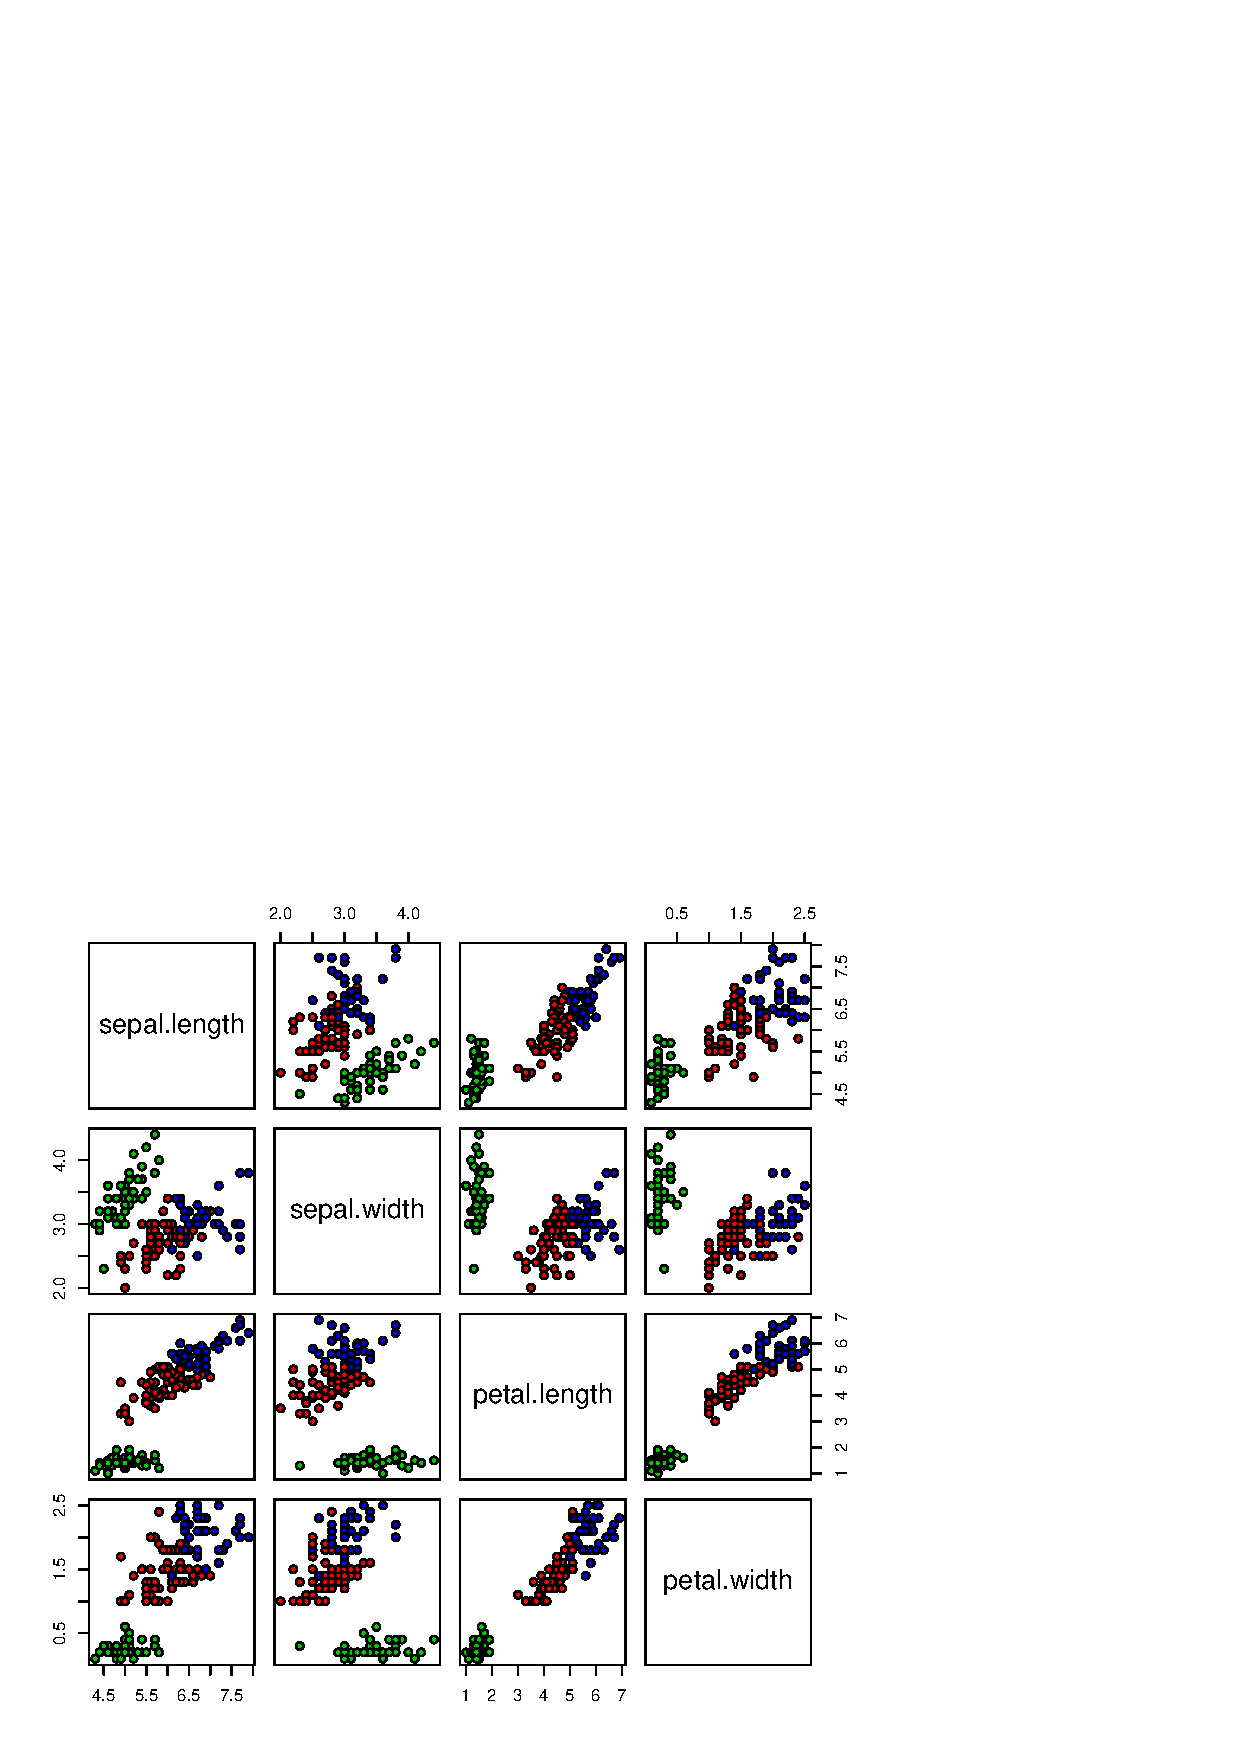
\includegraphics[width=0.8\textwidth]{images/ml/iris-flower-kmeans}
  \end{center}
  \caption{Визуализация клустеризации набора данных ``Ирисы Фишера''.}
  \label{ml:fig:iris-dataset-kmeans}
\end{figure}
}

\section{Классификация}
\emph{Классификация} объекта — это указание класса для данного объекта. Например, по значениям длин и ширин чашелистника и лепестка цветка ириса нужно определить его вид.

\subsection{Метод $k$ ближайших соседей}
Суть \emph{метода $k$ ближайших соседей} (англ. k-nearest neighbor algorithm) состоит в том, что объекту присваивается тот класс, который является наиболее распространённым среди его $k$ соседей. Из этого следует, что нужно иметь набор данных с заранее известными классами объектов.

Для определения близости, как правило, используется евклидова метрика.

Предельно наивная реализация данного алгоритма — предельно очевидна. Она же — приведена ниже:
\begin{pylst}{Наивная реализация kNN}{}
def knn(item, dataset):
    klass = None
    nearest = None

    for row in dataset:
        next = metrics.sim_distance(item, row["features"])

        if nearest is None:
            nearest =  next
        elif next > nearest:
            klass = row["class"]
            nearest = next

    return klass
\end{pylst}

Пример запуска для набора данных ``Ирисы Фишера'':
\begin{pylst}{}{}
>>> knn([4.5, 3.8, 1.2, 0.4], dataset)
"setosa"
\end{pylst}

\subsection{kd деревья}
\emph{kd дерево} (англ. k-dimensional tree) — структура данных, используемая для разбития $k$-размерного пространства на подпространства по некоторым заданных точкам.

kd дерево — это бинарное дерево, в котором каждый узел содержит точку пространства размерности $k$. Каждый внутренний узел представляет собой точку, через которую проходит гиперплоскость, разбивающая пространство на две части. При этом точки из левого поддерева находятся по одну сторону от этой гиперплоскости, точки же правого поддерева — по другую.

Направление гиперплоскостей выбирается следующим образом: выбирается какая-либо ось, и гиперплоскость строится перпендикулярно к этой оси. Например, допустим выбрана ось $x$, тогда все точки текущего поддерева, у которых координата по оси $x$ меньше, будут находится по одну сторону от гиперплоскости, проведённой через точку $(x_{concrete}, 0, \dots)$; оставшиеся же точки — по другую сторону. При этом первые — будут в левом поддереве, вторые же — в правом.

\subsubsection{Построение kd дерева}
Так как способов выбирать следующую ось, перпендикулярно которой строится следующая гиперплоскость, — много, то и построений может быть — много. Каноническим способом является:
\begin{itemize}
  \item Циклически и последовательно выбирать следующую ось по порядку, начиная с оси $x$, для каждого следующего уровня дерева.
  \item Элементом текущего узла является точка, которая является медианой точек текущего поддерева.
\end{itemize}

Посмотрим дерево для точек $(2; 3), (5; 4), (9; 6), (4; 7), (8; 1), (7; 2)$. Оно будет выглядеть, как на \autoref{ml:knn:kdtree-pic}. На плоскости же его можно изобразить, как на \autoref{ml:knn:kdtree-2d}.

Ниже приведена реализация построения kd дерева из массива вышеупомянутых точек.

\begin{pylst}{}{}
class Node(object):
    def __init__(self, location, left, right):
        self.location = location
        self.left = left
        self.right = right

def kdtree(points, depth=0):
    if not points.size:
        return None

    n, k = points.shape
    axis = depth % k

    points.sort(axis=axis)
    median = n // 2

    location = points[median]
    left = kdtree(points[:median], depth + 1)
    right = kdtree(points[median + 1:], depth + 1)
    node = Node(location, left, right)

    return node
\end{pylst}

\begin{figure}[htb]
  \centering
  \begin{tikzpicture}[xNode/.style={circle,draw,red},
                      yNode/.style={circle,draw,blue},
                      justNode/.style={circle,draw,black},
                      level distance=1.5cm,
                      level/.style={sibling distance=2.5cm/#1},
                      font=\footnotesize]
    \node [xNode] at (0,0) {$7; 2$}
      child { node [yNode] {$5; 4$}
        child { node [justNode] {$2; 3$} }
        child { node [justNode] {$4; 7$} } }
      child { node [yNode] {$9; 6$}
        child { node [justNode] {$8; 1$} } };
  \end{tikzpicture}
  \caption{Пример kd дерева.}
  \label{ml:knn:kdtree-pic}
\end{figure}

\begin{figure}[htb]
  \centering
  \begin{tikzpicture}
    \begin{axis}[
      xlabel=$x$,
      ylabel=$y$,
      xmin=0, xmax=10,
      ymin=0, ymax=10]

      \draw [red] (axis cs:7,0)
        -- (axis cs:7,10);

      \draw [blue] (axis cs:0,4)
        -- (axis cs:7,4);

      \draw [blue] (axis cs:7,6)
        -- (axis cs:10,6);

      \addplot[
        scatter/classes={
          x={mark=square*,red},%
          y={mark=square*,blue},%
          n={mark=square*,black}
        },
        scatter,only marks,
        scatter src=explicit symbolic]
        coordinates {
          (7,2) [x]
          (5,4) [y]
          (9,6) [y]
          (2,3) [n]
          (4,7) [n]
          (8,1) [n]
        };
    \end{axis}
  \end{tikzpicture}
  \caption{Изображение kd дерева на плоскости.}
  \label{ml:knn:kdtree-2d}
\end{figure}


\end{document}
